\chapter{Analiza}
\label{ch:analiza}

Svaki broj u ovoj glavi dolazi iz izmerenog pokretanja. Glava je duga, pa su njeni nalazi prvo sakupljeni ovde, svaki sa odeljkom koji ga utvr\dj{}uje.

\begin{itemize}
\item Sva \v{c}etiri efekta zajedno ko\v{s}taju \perfFourEffectsAMD{} ms na RX 9070 XT i
      \perfFourEffectsNV{} ms na RTX 5070, \v{s}to je na obe kartice unutar frejma od 60 Hz
      (Odeljak~\ref{sec:cena}).
\item Dve kartice se ne sla\v{z}u oko toga koji je efekat skup, a neslaganje dopire do in\v{z}enjerske odluke: od dve strategije za senke svaka je jeftinija na jednoj kartici
      (Odeljci~\ref{sec:cena} i \ref{sec:analiza-shadow-strategy}).
\item Vi\v{s}e zraka donosi veoma malo. Osam puta ve\'ci bud\v{z}et vra\'ca \rcPsnrGain{} dB PSNR-a za
      \rcGpuPct\% vi\v{s}e GPU vremena, pa je radna ta\v{c}ka jedan zrak po pikselu
      (Odeljak~\ref{sec:raycount}). Pra\'cenje u polovini rezolucije pona\v{s}a se isto
      (Odeljak~\ref{sec:halfres}).
\item Prostorni denoiser opravdava svoju cenu stabilno\v{s}\'cu, a ne ta\v{c}no\v{s}\'cu na mirnoj slici: stati\v{c}ke metrike pomera za manje od \v{s}uma merenja, a treperenje izme\dj{}u frejmova
      smanjuje za \flickerPct\% (Odeljci~\ref{sec:denoise-eval} i \ref{sec:motion}).
\item Pra\'cenje zraka najvi\v{s}e podi\v{z}e kvalitet tamo gde rasterizacija ima najmanje \v{s}ta da
      radi, pa FLIP pada sa \qRasterFlip{} na \qAllRtFlip{}, uz globalno osvetljenje kao dominantan \v{c}lan
      (Odeljak~\ref{sec:poredjenje}).
\item Ugradnja ray query-ja u liniji ko\v{s}ta zauzetost: forward \v{s}ejder prelazi sa 87 na 130 registara, a sa
      16 istovremeno rezidentnih talasa na 10 (Odeljak~\ref{sec:occupancy}).
\end{itemize}

Dve stvari se ponavljaju i ovde se navode jednom, umesto u svakom odeljku. Cene se \v{c}itaju sa \emph{lestvice} konfiguracija, gde svaka \emph{prečka} dodaje jedan efekat, pa je cena efekta
razlika izme\dj{}u susednih pre\v{c}ki. I svaka razlika se \v{c}ita naspram praga ponovljivosti
utvr\dj{}enog u Odeljku~\ref{sec:metodologija}, ispod kog ovaj protokol ne mo\v{z}e da razdvoji dve
konfiguracije, zbog \v{c}ega je nekoliko rezultata ispod prijavljeno kao nepostojanje razlike, a ne kao
mala razlika.

\section{Metodologija}
\label{sec:metodologija}

\paragraph{Hardver: me\dj{}uvendorska postavka.} Centralna evaluacija poredi identi\v{c}an pipeline na
dve grafi\v{c}ke kartice aktuelne generacije od razli\v{c}itih proizvo\dj a\v{c}a: AMD Radeon RX 9070 XT (RDNA4) i NVIDIA
GeForce RTX 5070 (Blackwell), navedene u Tabeli~\ref{tab:gpus}. Obe pokre\'cu isti binarni fajl engine-a,
iste SPIR-V \v{s}ejdere, isti graf renderovanja i istu scenu sa istim pode\v{s}avanjima. Jedina promenljiva je
izabrani fizi\v{c}ki ure\dj{}aj, \v{s}to je osnova poštenja: svaka razlika u vremenu poti\v{c}e od
hardvera i drajvera, a ne od druge putanje koda, dok bi razilaženje kvaliteta ukazivalo na
nedeterminizam vredan istrage, a ne na stvarnu razliku. Jedini dokumentovani izuzetak od tvrdnje o identi\v{c}noj putanji koda je podr\v{s}ka za opacity micromap.

\begin{table}[tbp]
\caption[Grafi\v{c}ke kartice u me\dj{}uvendorskom poređenju]{Grafi\v{c}ke kartice u me\dj{}uvendorskom poređenju, prema slu\v{z}benim specifikacijama proizvo\dj a\v{c}a
(AMD, NVIDIA) i verzijama drajvera na ma\v{s}ini za testiranje.}
\label{tab:gpus}
\centering
\begin{tabularx}{\textwidth}{l >{\raggedright\arraybackslash}X >{\raggedright\arraybackslash}X}
\toprule
 & AMD RX 9070 XT & NVIDIA RTX 5070 \\
\midrule
Arhitektura            & RDNA4 (Navi 48) & Blackwell (GB205) \\
Compute jedinice / SM  & 64 CU, 4096 stream procesora & 48 SM, 6144 CUDA jezgra \\
RT akceleratori        & 64 (3. generacija) & 48 \\
Takt (boost)           & 2970 MHz & 2512 MHz \\
Memorija / propusnost  & 16 GB GDDR6, 640 GB/s & 12 GB GDDR7, 672 GB/s \\
TDP (TBP / TGP)        & 304 W & 250 W \\
Drajver / OS           & 32.0.31035.1003, Windows 11 Pro (build 26100) & 32.0.15.9186, Windows 11 Pro (build 26100) \\
\bottomrule
\end{tabularx}
\end{table}

Dva reda koja najvi\v{s}e li\v{c}e na rang-listu su ona koja se najmanje mogu porediti. Stream procesor
i CUDA jezgro nisu ista jedinica posla, pa 4096 prema 6144 nije faktor 1.5 ni u \v{c}emu, a broj RT
akceleratora ima razli\v{c}it smisao kod svakog proizvo\dj a\v{c}a upravo zato \v{s}to dva proizvo\dj a\v{c}a razli\v{c}ito dele
obilazak (Odeljak~\ref{sec:accel-pregled}). Kartice su uparene po onome \v{s}to se mo\v{z}e porediti:
propusnost memorije u okviru 5\%, ista generacija procesa i susedni polo\v{z}aji u linijama proizvoda. Gde se u merenjima koja slede razilaze,
strukturni kandidat je ta podela obilaska, a ne bilo koji pojedinačni broj iz ove tabele, a
Odeljak~\ref{sec:cena} pokazuje da odnos po prolazu obuhvata raspon od \perfRatioMin{} do \perfRatioMax{}, koji nijedna
pojedina\v{c}na hardverska vrednost ne mo\v{z}e da proizvede.

\paragraph{Nepodudaranje podr\v{s}ke za OMM.} Sponza ima tri MASK materijala (alfa-isecanje), koji se prate
kroz opacity-micromap BLAS na ure\dj{}aju koji izla\v{z}e \texttt{VK\_EXT\_opacity\_micromap}, a inače
kroz rezervni any-hit alfa-test (Odeljak~\ref{sec:accel}). Drajver RTX 5070 izla\v{z}e ekstenziju, a drajver 9070 XT ne, uprkos uporedivim hardverskim mogu\'cnostima, pa
dva proizvo\dj a\v{c}a ovde razre\v{s}avaju maskiranu geometriju kroz zaista razli\v{c}it kod strukture ubrzanja. Ta
razlika menja samo na\v{c}in na koji se maskirani mikrotrougao klasifikuje tokom obilaska, a ne pravac zraka,
poziciju pogotka ni \v{s}ejding, pa je lo\v{s} kandidat za razliku u metrici kvaliteta: pe\v{c}enje je
konzervativno i svaki mikrotrougao \v{c}iji se barycentric uzorci ne sla\v{z}u \v{s}alje u stanje
\texttt{UNKNOWN} koje i dalje izvr\v{s}ava ta\v{c}an any-hit alfa-test, pa do rezolucije te mre\v{z}e uzoraka
ekstenzija menja koliko obilazak ko\v{s}ta, a ne \v{s}ta nalazi. To je mali jednosmerni doprinos koji zavisi od drajvera, u razlici u GPU-ms po efektu gde god zrak pogodi isečenu
geometriju, i ova evaluacija ga dalje ne izoluje.

\paragraph{Scena i kontrole.} Test scena je Sponza, standardni enterijer sa jakim indirektnim
odbijanjem, osvetljen sa pet uklju\v{c}enih svetala: \v{c}etiri ta\v{c}kasta (baklje) i jedno usmereno (sunce). Tri reflektorska svetla i
dva dodatna ta\v{c}kasta su definisana ali isklju\v{c}ena, a razlika je bitna jer podrazumevana
putanja senki ko\v{s}ta dva zraka po svetlu po pikselu.

Jedno svojstvo rasterske putanje ograni\v{c}ava svaku tehniku koja je koristi: engine alocira najvi\v{s}e dve
omni mape senki (\texttt{MAX\_SHADOW\_POINTS}, \v{s}est prolaza dubine svaka), pa dva od \v{c}etiri uklju\v{c}ena
ta\v{c}kasta svetla renderuju bez senke. Senke sa pra\'cenjem zraka nemaju takvo ograni\v{c}enje i prate svako svetlo, pa
svaka tehnika u Tabeli~\ref{tab:quality} osim \texttt{all-RT} stoji na slabijoj osnovi senki
nego renderer bez tog ograni\v{c}enja, \v{s}to ide u korist strane sa pra\'cenjem zraka. Efekat je ograni\v{c}en i
mali: sama tehnika senki pomera PSNR za 0.65 dB od \qRtLiftPsnr{} dB izme\dj{}u rastera i svih efekata,
a FLIP za 0.024 od 0.349, pa u pobolj\v{s}anju iz Odeljka~\ref{sec:poredjenje} dominira globalno
osvetljenje, a ne ovo ograni\v{c}enje.

Dve porodice merenja u ovoj glavi ne dele rezoluciju, jer se izvode na razli\v{c}itim mestima. Vremena dolaze iz editora u
$\perfWidth{} \times \perfHeight{}$, veli\v{c}ini koju svaka osnovna linija bele\v{z}i kako bi se pokretanje u drugoj
preskakalo umesto upore\dj ivalo, dok snimci kvaliteta koriste runtime bez editora i
pre ocenjivanja se resampluju na kanonsku veli\v{c}inu. Zato se cene porede sa cenama, a ocene sa ocenama, nikad
me\dj{}usobno. Za svako A/B kamera je statična,
jer pokretna kamera desinhronizuje niz frejmova izme\dj{}u dva pokretanja i izmi\v{s}lja razlike koje su
artefakti vremena. Ke\v{s} \v{s}ejdera se bri\v{s}e pre nego \v{s}to se poveruje bilo kojoj GPU metrici, jer
zastareo ke\v{s} daje nedeterministi\v{c}ke rezultate, a sa\v{c}uvane konzolne promenljive se tokom benchmark pokretanja ignori\v{s}u, pa preostalo pode\v{s}avanje ne mo\v{z}e neprimetno da promeni konfiguraciju.

\paragraph{Merenje performansi.} GPU vreme dolazi iz timestamp opsega po prolazu i
\texttt{perf-bench} alata iz Odeljka~\ref{sec:alati}, usrednjeno preko fiksnog bud\v{z}eta frejmova kad se
stabilno stanje detektuje, a ne pretpostavi: vreme frejma se na ovoj sceni sti\v{s}ava tek posle oko pedeset frejmova, pa bi
fiksno kratko zagrevanje u rezultat usrednjilo deo rasta takta, u iznosu koji zavisi od toga koliko je ma\v{s}ina ve\'c bila topla, bez ikakvog traga u izlazu.
Benchmark prolazi fiksnu matricu konfiguracija, uklju\v{c}uju\'ci po jedan efekat vi\v{s}e u svakom koraku, pa je
cena efekta razlika izme\dj{}u susednih (Tabela~\ref{tab:cena}). Razlika, a ne izolovano merenje, jer
efekti dele fiksni posao: struktura ubrzanja se gradi jednom, G-bafer se puni jednom, tonemap se izvr\v{s}ava jednom, pa bi merenje jednog efekta samog njemu
naplatilo sve to i \v{c}etiri vrednosti bi u zbiru daleko prelazile frejm. Razlika se uzima na \emph{ukupnom}
GPU vremenu, a ne na opsegu jednog prolaza, jer se inline senke prate unutar Forward prolaza i
nemaju sopstveni, a ostala tri se prijavljuju isto radi doslednosti. Timestampovi se
pretvaraju periodom timestampa svakog ure\dj{}aja, pa su vremena po prolazu uporediva izme\dj{}u proizvo\dj a\v{c}a.

\paragraph{Merenje kvaliteta.} Kvalitet rekonstrukcije meri \texttt{quality-bench} naspram
konvergirane path-traced reference iz Odeljka~\ref{sec:pathtracer}. Tonemapirani prikaz svake tehnike u realnom vremenu
ocenjuje se naspram nje merom \textbf{FLIP} (perceptivna) \cite{andersson2020flip},
\textbf{PSNR} i \textbf{SSIM} \cite{wang2004ssim}. FLIP je primarna jer modeluje ono \v{s}to posmatra\v{c}
primećuje, a ne sirovu gre\v{s}ku po pikselu. PSNR strukturno favorizuje zamu\'cenu sliku, a SSIM poredi lokalnu strukturu, a ne
apsolutne vrednosti, pa se prijavljuju sve tri i nijedna pristrasnost jedne metrike ne odlu\v{c}uje o zaklju\v{c}ku.
Ocene se usrednjuju preko tri fiksne orijentacije iz jedne unutra\v{s}nje pozicije (niz glavni brod, nagnuto
ka podu, nagnuto ka gornjoj galeriji), izabrane tako da razli\v{c}ito optere\'cuju ambijentalnu okluziju, globalno osvetljenje
i refleksije, pa jedno kadriranje ne mo\v{z}e da pristrasno utiče na rezultat. Svaki snimak se prvo bilinearno
resamplira na kanonsku $1024 \times 576$, pa razlika u veli\v{c}ini prozora izme\dj{}u pokretanja ne mo\v{z}e neprimetno da promeni ocenu. Vrednosti kvaliteta na drugim mestima u ovoj glavi
su sa RX 9070 XT, iako Odeljak~\ref{sec:cross-vendor-quality} snima celu matricu i na
RTX 5070.

Ova glava koristi ukupno \v{s}est mera, tri za mirnu sliku i tri koje zahtevaju kretanje.
Tabela~\ref{tab:metrics} ih sakuplja, sa smerom u kom se pobolj\v{s}avaju i najmanjom
razlikom koju ovaj protokol mo\v{z}e da razre\v{s}i, da \v{c}italac koji na neku naiđe kasnije ne mora
da je rekonstrui\v{s}e iz teksta u kom je uvedena.

\begin{table}[tbp]
\caption[Mere kori\v{s}\'cene u ovoj glavi]{Mere kori\v{s}\'cene u ovoj glavi i najmanja
razlika koju svaka mo\v{z}e da razre\v{s}i. Tri praga su ponovljivost, izmerena ponovnim snimanjem cele
matrice i o\v{c}itavanjem koliko su se pet tehnika koje nisu mogle da se promene ipak pomerile
(petnaest snimaka), metodom iz pasusa ispod. Mere kretanja nemaju sopstveni prag
ovde, jer su snimljene jednom, a ne ponovo.}
\label{tab:metrics}
\centering
\small
\begin{tabularx}{\textwidth}{@{}l>{\raggedright\arraybackslash}X c r@{}}
\toprule
Mera & \v{S}ta poredi & Bolje & Prag \\
\midrule
FLIP  & frejm naspram path-traced reference, ponderisano onim \v{s}to posmatra\v{c} primeti\'ce & ni\v{z}e & 0.0024 \\
PSNR  & isto, kao logaritam srednje kvadratne gre\v{s}ke, \v{s}to favorizuje zamu\'cenu sliku & vi\v{s}e & 0.06 dB \\
SSIM  & isto, kao lokalna struktura, a ne apsolutne vrednosti piksela & vi\v{s}e & 0.0022 \\
\addlinespace[3pt]
tFLIP & koliko se tehnika menja izme\dj{}u susednih frejmova, preko onoga koliko se referenca menja u istom intervalu & ni\v{z}e & -- \\
kašnjenje & pokretni frejm naspram sopstvenog konvergiranog mirnog frejma ovog renderera u istoj pozi & ni\v{z}e & -- \\
JOD   & ColorVideoVDP, jedina mera ovde koja direktno modeluje temporalnu osetljivost na kontrast, gde je 1 JOD otprilike 75\% preferencije populacije & vi\v{s}e & -- \\
\bottomrule
\end{tabularx}
\end{table}

Nekoliko rezultata ispod zavisi od razlike koja je premala da bi se pro\v{c}itala, pa ti pragovi moraju
odnekud da dođu. Ponovno snimanje cele matrice posle promene denoisera daje ih bez posebnog
eksperimenta: pet tehnika (\texttt{raster}, \texttt{ssao}, \texttt{ssr}, \texttt{rtao},
\texttt{rtrefl}) ne izvr\v{s}ava filter koji se promenio, pa je ono za \v{s}ta su se njihove ocene pomerile
ponovljivost, a ne efekat. Tri koje ga izvr\v{s}avaju pomerile su se do 0.0096 FLIP, \v{c}etiri puta vi\v{s}e od
praga, \v{s}to je razdvajanje koje metodu \v{c}ini vrednom. To je jedno ponovno snimanje, a ne
studija ponovljenih merenja, pa vrednosti iz Tabele~\ref{tab:metrics} treba \v{c}itati kao pravi red
veli\v{c}ine, a ne kao intervale poverenja.

\section{Cena po efektu (GPU ms)}
\label{sec:cena}

\begin{table}[tbp]
\caption[Cena po efektu na oba adaptera]{Cena po efektu (GPU ms) na me\dj{}uvendorskom paru RX 9070 XT / RTX 5070, pri
$\perfWidth \times \perfHeight$ sa fiksnom pozom kamere, usrednjeno preko \perfFrames{} frejmova.
\texttt{rt-off} je ukupno GPU vreme bez RT efekata, a svaki red iznad prve linije je delta tog
efekta nad konfiguracijom navedenom u prethodnom redu. Tri bloka odgovaraju na razli\v{c}ita
pitanja: lestvica daje cenu svakog efekta sa pra\'cenjem zraka, srednji red daje cenu gotovog
frejma kad su sva \v{c}etiri uklju\v{c}ena, a poslednji blok daje cenu screen-space alternative svakog od
tri efekta koji je imaju. To nisu dalje pre\v{c}ke, pa se svaka oduzima od iste osnove
kao njen parnjak sa pra\'cenjem zraka, a ne nadovezuje na njega, \v{s}to ih \v{c}ini direktno
uporedivim. Sve vrednosti generi\v{s}e \texttt{tools/gen\_perf\_tables.py} iz commitovanih osnovnih linija.}
\label{tab:cena}
\centering
\input{data/perf-effects.tex}
\end{table}

U Tabeli~\ref{tab:cena} redovi po efektu su razlike, dok je ukupno izmereno vreme celog frejma
konfiguracije \texttt{+gi}, a ne njihov zbir, pa se zaokru\v{z}ivanje ne mo\v{z}e nagomilati.
Tabela~\ref{tab:pass-cost} razla\v{z}e isti frejm po prolazima.

\begin{table}[tbp]
\caption[Najskuplji prolazi sa uklju\v{c}enim RT GI]{Najskuplji prolazi u konfiguraciji \texttt{+gi} (GPU ms, usrednjeno preko
\perfFrames{} frejmova). \texttt{Forward} nosi i inline RT senke, pa one nemaju sopstveni opseg. GI i AO filtriraju u polovini rezolucije. Prolazi denoise refleksija nisu u
tabeli jer se vi\v{s}e ne izvr\v{s}avaju: \texttt{render.reflections.denoise.iterations} je sada 0
(Odeljak~\ref{sec:denoise-eval}).}
\label{tab:pass-cost}
\centering
\input{data/perf-passes.tex}
\end{table}


\begin{figure}[tbp]
\centering
\begin{tikzpicture}
\begin{axis}[width=0.88\textwidth, height=6.4cm,
  xlabel={konfiguracija}, ylabel={ukupno GPU (ms)},
  xtick={0,1,2,3,4},
  xticklabels={\texttt{rt-off},\texttt{shadows},\texttt{+ao},\texttt{+refl},\texttt{+gi}},
  ymin=0, grid=major, grid style={black!12},
  tick label style={font=\small}, label style={font=\small},
  legend style={at={(0.02,0.98)}, anchor=north west, font=\small, draw=black!30}]
\addplot[thick, mark=*] table[col sep=tab, x=i, y=amd] {data/ladder.dat};
\addplot[thick, mark=square*, dashed] table[col sep=tab, x=i, y=nv] {data/ladder.dat};
\legend{RX 9070 XT, RTX 5070}
\end{axis}
\end{tikzpicture}
\caption[Kumulativno GPU vreme preko lestvice konfiguracija]{Ukupno GPU vreme preko lestvice, gde
svaka sledeća konfiguracija uklju\v{c}uje jo\v{s} jedan efekat. Nagib segmenta je cena tog efekta. Obe kartice
rastu monotono, iako AMD po\v{c}inje vi\v{s}e i br\v{z}e raste, pa se razlika pove\'cava sa
\perfGapBase{} ms pri \texttt{rt-off} na \perfGapGi{} ms pri \texttt{+gi}.}
\label{fig:ladder}
\end{figure}

\begin{figure}[tbp]
\centering
\begin{tikzpicture}
\begin{axis}[xbar, bar width=5pt, width=0.62\textwidth, height=9.5cm,
  xlabel={odnos AMD / NVIDIA (GPU ms)},
  xmin=0, xmax=2.2, y dir=reverse,
  ytick={0,...,15}, yticklabels from table={data/passcost-vendor.dat}{pass},
  yticklabel style={font=\footnotesize}, tick label style={font=\small},
  label style={font=\small}, grid=major, grid style={black!12},
  nodes near coords, nodes near coords style={font=\tiny, /pgf/number format/fixed,
    /pgf/number format/precision=2}]
\addplot[fill=black!18, draw=black!55] table[col sep=tab, x=ratio, y expr=\coordindex]
  {data/passcost-vendor.dat};
\draw[dashed, black!60] (axis cs:1,-1) -- (axis cs:1,16);
\end{axis}
\end{tikzpicture}
\caption[Odnos cene po prolazu izme\dj{}u proizvo\dj a\v{c}a]{Cena svakog prolaza na AMD podeljena cenom istog prolaza
na NVIDIA, u konfiguraciji \texttt{+gi}. Isprekidana linija je parnost. Desno od nje NVIDIA je
br\v{z}a, levo AMD. Raspon od \perfRatioMin{} do \perfRatioMax{} pokazuje da razlika nije jedan globalni faktor takta:
\texttt{Forward} (koji nosi inline senke), \texttt{GI} trace i prva a-trous
iteracija snažno idu u prilog NVIDIA-i, dok treća a-trous iteracija i \texttt{DepthNormal} idu u prilog
AMD-u.}
\label{fig:vendor-ratio}
\end{figure}

Obe kartice se sla\v{z}u oko najskupljeg efekta, \perfTopEffectAMD{} na RX 9070 XT
(\perfEffShadowsAMD{} ms) i \perfTopEffectNV{} na RTX 5070 (\perfEffShadowsNV{} ms), i oko
najjeftinijeg, ambijentalne okluzije. Ispod vrha ne daju isti redosled, a merenje
razre\v{s}ava samo njegov deo. Svaka cena je razlika dve konfiguracije, pa nosi rasipanje izme\dj{}u
pokretanja obe konfiguracije. Na 9070 XT senke prevazilaze to rasipanje, dok su
\perfUnresolvedAMD{} udaljeni \perfUnresolvedGapAMD{} ms, unutar njega. Na 5070 senke ga ne prevazilaze
u odnosu na globalno osvetljenje (\perfEffGiNV{} ms), udaljeno \perfUnresolvedGapNV{} ms, pa je
vrh rang-liste 5070 izjedna\v{c}en, a redosled efekata ispod njega (globalno osvetljenje iznad
refleksija sa \perfEffReflNV{} ms) jedini je koji ona podr\v{z}ava. Sva \v{c}etiri zajedno ko\v{s}taju \perfFourEffectsAMD{} i
\perfFourEffectsNV{} ms, za ukupno \perfTotalAMD{} i \perfTotalNV{} ms, \v{s}to je na obe unutar
16.7 ms frejma od 60 Hz i \v{c}ini tvrdnju o realnom vremenu merenjem, a ne oznakom.
Slika~\ref{fig:ladder} crta lestvicu, a Slika~\ref{fig:effect-gallery} pokazuje \v{s}ta svaki efekat
doprinosi slici.

Tri od \v{c}etiri rang-liste slede iz toga kuda zraci idu. GI i AO ostaju jeftini uprkos prikupljanju preko
hemisfere jer oba prate i uklanjaju \v{s}um u polovini rezolucije, a AO je najjeftiniji uprkos tome \v{s}to
baca najvi\v{s}e zraka po pikselu, jer su njegovi zraci ograni\v{c}eni sa \texttt{render.ao.radius} i
zavr\v{s}avaju se na prvom pogotku, dok zrak refleksije mo\v{z}e da pre\dj e scenu i zatim \v{s}ejdira ono \v{s}to na\dj e.
Refleksije su jedini efekat koji i dalje prati u punoj rezoluciji, a to \v{s}to vi\v{s}e nisu najskuplje
je promena podrazumevane vrednosti, a ne optimizacija: njihov à-trous se pokazao neto negativnim i
sada izvr\v{s}ava nula iteracija (Odeljak~\ref{sec:denoise-eval}), \v{s}to uklanja lanac od tri prolaza u punoj rezoluciji. Svaki efekat sa screen-space alternativom jeftiniji je u tom obliku, na obe kartice, ali ne
za jedan faktor: \perfSsFactorMin{} do \perfSsFactorMax{} puta (Tabela~\ref{tab:cena}), od
\perfSsFactorGiNV{} za globalno osvetljenje na 5070 do \perfSsFactorReflAMD{} za refleksije na
9070 XT. Taj faktor je cena pitanja o geometriji van ekrana i stabilna je polovina
poređenja, jer nikad ne pada ispod \perfSsFactorMin{}. Da li se isplati
je pitanje za Odeljak~\ref{sec:poredjenje}, gde se pokazuje da odgovor potpuno zavisi od toga za koji se
efekat pla\'ca.

Senke se \v{c}itaju preko konfiguracija, a ne iz prolaza, jer nemaju sopstveni opseg, i
njihovi \v{c}lanovi po prolazu se ne zatvaraju sasvim. Izme\dj{}u \texttt{rt-off} i \texttt{shadows} na 9070 XT
Forward prolaz raste za \perfFwdGrowAMD{} ms dok rasterski prolazi senki (\texttt{Shadow} i
\texttt{PointShadows}) vra\'caju \perfShadowMapsAMD{} ms, \v{s}to daje \perfPassNetAMD{} ms naspram izmerene
razlike celog frejma od \perfEffShadowsAMD{} ms. Preostalih \perfPassResidAMD{} ms su istovremeno smanjivanje ostalih
prolaza i vreme izvan svakog opsega prolaza, \v{s}to je pomeranje takta, a ne
u\v{s}teda, pa je razlika celog frejma broj koji treba navoditi.

\begin{figure}[tbp]
\centering
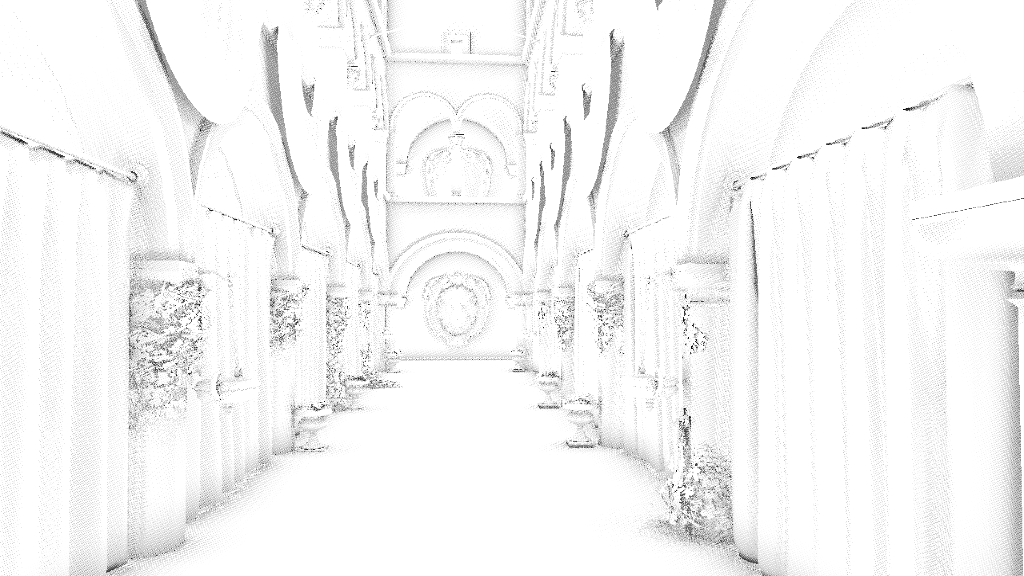
\includegraphics[width=0.48\textwidth]{figures/dbg_ao.png}\hfill%
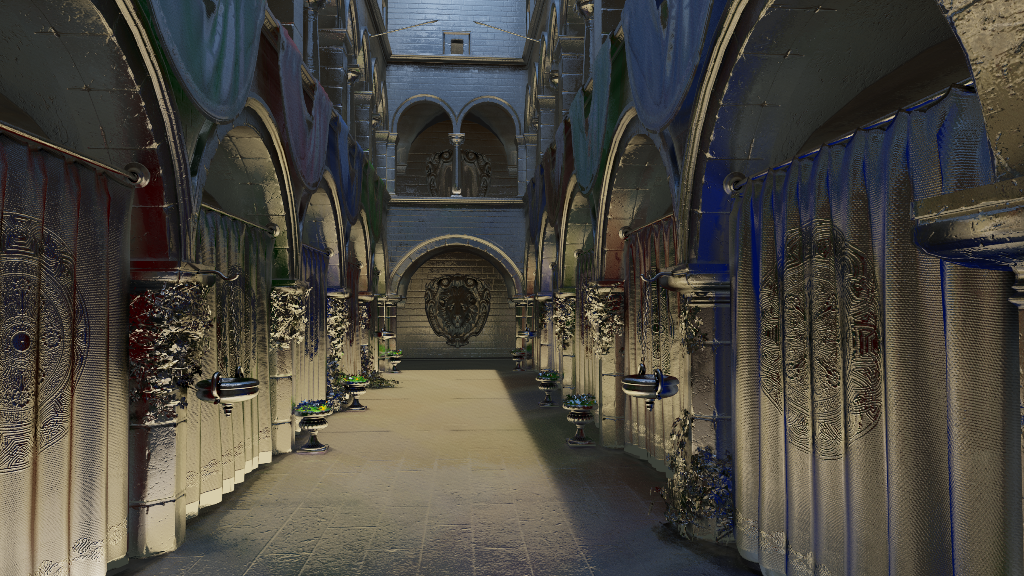
\includegraphics[width=0.48\textwidth]{figures/dbg_refl.png}

\vspace{5pt}

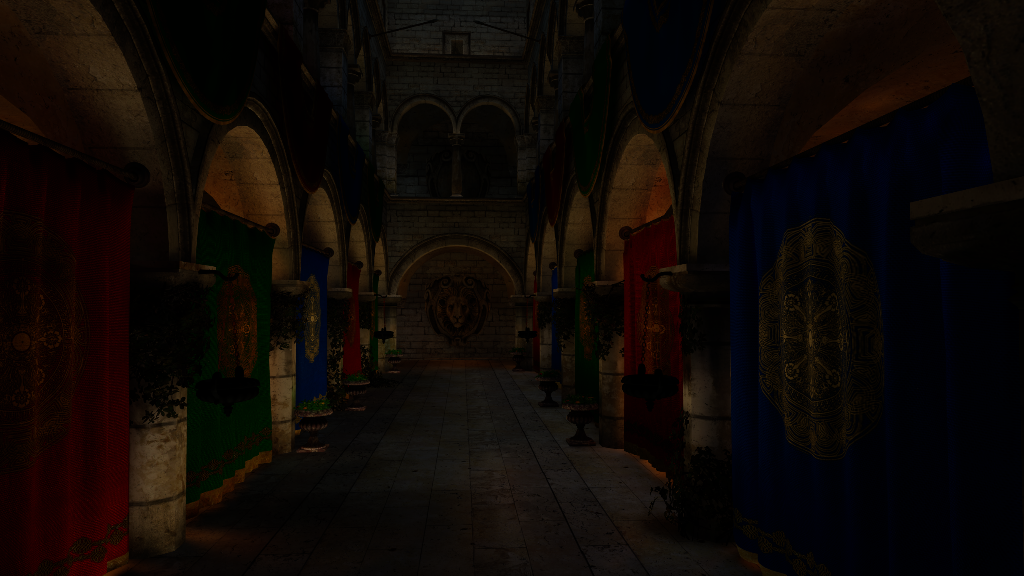
\includegraphics[width=0.48\textwidth]{figures/dbg_gi.png}\hfill%
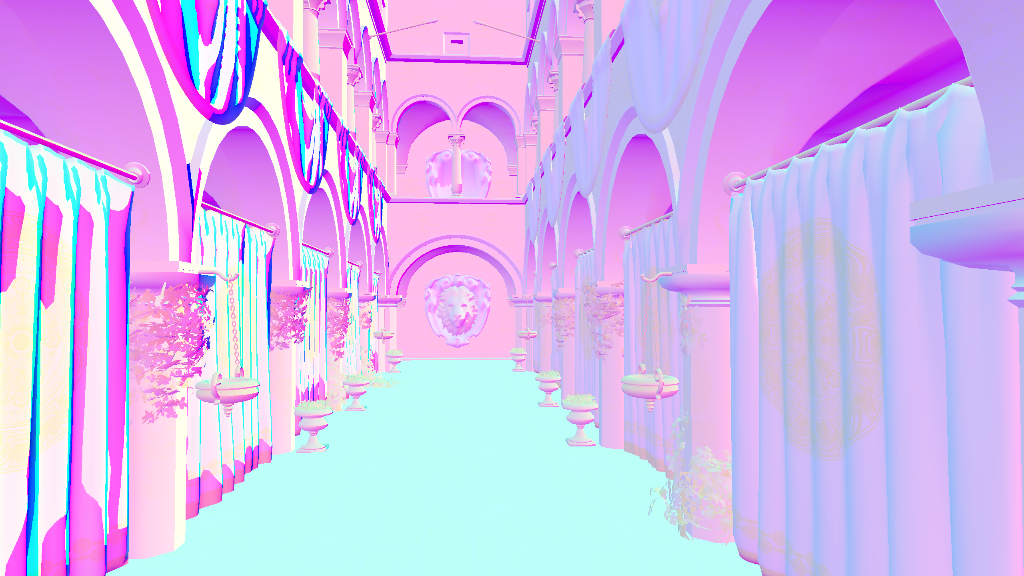
\includegraphics[width=0.48\textwidth]{figures/dbg_normals.png}
\caption[Pojedina\v{c}ni signali izolovani debug prikazom]{Pojedina\v{c}ni signali izolovani kroz \texttt{render.debugview}, ista scena i kamera: ambijentalna
okluzija (gore levo), reflektovana radijansa (gore desno), indirektni GI \v{c}lan (dole levo) i normale G-bafera
(dole desno). To su sirovi me\dj{}urezultati pre nego \v{s}to se u forward prolazu kombinuju,
a ne gotova slika.}
\label{fig:effect-gallery}
\end{figure}

Globalno osvetljenje je jedini od \v{c}etiri efekta koji znatno menja sliku.
Pojedina\v{c}no uklju\v{c}ivanje senki, ambijentalne okluzije ili refleksija pomera kona\v{c}nu sliku za prosek od
2.1 do 2.5 nivoa od 255 sa ovog gledi\v{s}ta, dok je globalno osvetljenje pomera za 23.9, faktor
deset. Bafer
ambijentalne okluzije je skoro beo preko ve\'ceg dela frejma jer je atrijum Sponze otvoren, pa je
okluzija ograni\v{c}ena na svodove arkada i podno\v{z}ja stubova. Sirovi GI \v{c}lan je u apsolutnom iznosu taman,
ali nosi preliv boja (crvene i zelene zavese koje boje kamen pored sebe) koji konstantan ambijent ne mo\v{z}e da reprodukuje.

\paragraph{Dva upozorenja ograni\v{c}avaju odnose izme\dj{}u proizvo\dj a\v{c}a.} Prvo je da oni nisu svojstva
\v{s}ejdera. Tri a-trous reda na Slici~\ref{fig:vendor-ratio} su jedan \v{s}ejder pokrenut tri puta sa
sve \v{s}irim korakom uzorkovanja, a odnos pada preko njih sa \perfAtrousGIFirst{} na \perfAtrousGILast{} na GI lancu (\perfAtrousAOFirst{} na \perfAtrousAOLast{} na AO). Kontrolisani
eksperiment na lancu denoisa senki, koji izvr\v{s}ava isti \v{s}ejder, razdvaja dve stvari
koje se razlikuju izme\dj{}u tih redova. Kad se jezgro dr\v{z}i uniformnim, a menja samo unutra\v{s}nja rezolucija, odnos izme\dj{}u prve i tre\'ce iteracije je \(1.02\) u punoj rezoluciji i \(0.47\) u polovini, a
sa jezgrom veli\v{c}ine penumbre je \(1.20\) i \(0.65\). Obe grane u punoj rezoluciji su ravne, a
obe grane u polovini rezolucije se invertuju, pa ga pokre\'ce rezolucija na kojoj lanac radi, a ne
jezgro, a uniformna grana u polovini rezolucije reprodukuje GI i AO lance (\(0.47\) naspram
\perfAtrousGIDrop{} i \perfAtrousAODrop{}, isti pad od prve do tre\'ce \v{c}itan iz osnovnih linija \texttt{+gi}). Za\v{s}to bi manji radni skup trebalo da obrne redosled proizvo\dj a\v{c}a ovde nije izolovano i
zahtevalo bi hardverske brojače, a ne timestampove. Eksperiment ipak utvr\dj{}uje da se odnos
proizvo\dj a\v{c}a po prolazu mora navoditi sa rezolucijom pri kojoj je izmeren, jer se isti kod
invertuje preko te jedne promenljive (tri pokretanja po grani, medijane, RX 9070 XT naspram RTX 5070).

Drugo ograni\v{c}ava sam argument o obilasku. Odeljak~\ref{sec:accel-pregled} nudi
petlju obilaska vo\dj enu \v{s}ejderom kao strukturni razlog da se o\v{c}ekuje da posao sa zracima ko\v{s}ta vi\v{s}e na RDNA,
a podela po prolazima je s tim u skladu, jer prolazi koji prate imaju prose\v{c}an odnos \perfVendorTracingMean{} naspram
\perfVendorOtherMean{} za sve ostale prolaze. To ipak ne obja\v{s}njava razliku celog frejma, a
lestvica to ka\v{z}e. RX 9070 XT je \perfLadderRatioShadows{} puta sporija od RTX 5070 na pre\v{c}ki \texttt{shadows}
i \perfLadderRatioGi{} puta sporija na \texttt{+gi}, pa se razlika \emph{smanjuje} kako se pra\'cenje zraka dodaje, a
sam posao sa pra\'cenjem zraka (ukupno \texttt{+gi} minus ukupno \texttt{rt-off}) nosi odnos od
\perfRtOnlyRatio{} naspram \perfLadderRatioBase{} za frejm bez pra\'cenja zraka. Da je obilazak vo\dj en \v{s}ejderom
dominantan \v{c}lan, dodavanje pra\'cenja zraka trebalo bi da pove\'ca razliku, a ne da je zatvara. Po\v{s}teno \v{c}itanje je
da je ovaj engine uop\v{s}te sporiji na ovoj AMD kartici iz razloga koje merenje ne identifikuje,
i da se kazna ne koncentri\v{s}e u pra\'cenju zraka. Pre\v{c}ka \texttt{rt-off} je najmanje
pouzdana od ovih vrednosti, sa \perfSpreadBaseAMD{}\% rasipanja izme\dj{}u pokretanja naspram \perfSpreadBaseNV{}\% na NVIDIA strani, iz
razloga datog u Odeljku~\ref{sec:metodologija}, iako trend pre\v{z}ivljava i bez nje, jer se dve
pre\v{c}ke sa obe njene strane rasipaju najvi\v{s}e \perfSpreadNeighbourMax{}\% na bilo kojoj kartici.

\section{Dve strategije senki: inline naspram stohasti\v{c}ke}
\label{sec:analiza-shadow-strategy}

Dve strategije senki iz Odeljka~\ref{sec:senke} imaju razli\v{c}ito oblikovane krive cene: podrazumevana
inline putanja prati dva zraka po svetlu po pikselu unutar forward \v{s}ejdera, dok stohasti\v{c}ka
bira jedno svetlo po pikselu resampliranim uzorkovanjem po zna\v{c}aju i rekonstrui\v{s}e rezultat zajedni\v{c}kim
denoiserom. Tabela~\ref{tab:shadow-strategy} meri obe na istoj sceni.

\begin{table}[tbp]
\caption[Cena inline naspram stohasti\v{c}kih senki]{Dve strategije senki na istoj sceni sa pet uklju\v{c}enih svetala (GPU ms, delta nad
\texttt{rt-off}).}
\label{tab:shadow-strategy}
\centering
\input{data/perf-shadow-strategy.tex}
\end{table}

\begin{figure}[tbp]
\centering
\begin{tikzpicture}
\begin{axis}[width=0.7\textwidth, height=6.0cm,
  xlabel={adapter}, ylabel={cena nad \texttt{rt-off} (GPU ms)},
  xtick={0,1}, xticklabels={RX 9070 XT, RTX 5070},
  xmin=-0.3, xmax=1.3, ymin=0, ymax=4,
  grid=major, grid style={black!12},
  tick label style={font=\small}, label style={font=\small},
  legend style={at={(0.02,0.98)}, anchor=north west, font=\small, draw=black!30}]
\addplot[thick, mark=*] table[x=i, y=inline] {data/shadow-strategy.dat};
\addplot[thick, mark=square*, dashed] table[x=i, y=stochastic] {data/shadow-strategy.dat};
\legend{inline, stochastic}
\end{axis}
\end{tikzpicture}
\caption[Cena strategije senki se obr\'ce izme\dj{}u proizvo\dj a\v{c}a]{Linije se seku. Na 9070 XT
stohasti\v{c}ka putanja je jeftinija, dok je na 5070 inline putanja jeftinija za faktor
\perfShadowRatioNV{}. Nijedan redosled se ne uop\v{s}tava.}
\label{fig:shadow-strategy}
\end{figure}

Dve kartice se ne sla\v{z}u oko toga koja je strategija jeftinija, a Slika~\ref{fig:shadow-strategy} pokazuje
kako se linije seku. Na RX 9070 XT stohasti\v{c}ka putanja pobe\dj uje,
\perfShadowStochAMD{} ms naspram \perfShadowInlineAMD{} ms. Na RTX 5070 jako gubi,
\perfShadowStochNV{} ms naspram \perfShadowInlineNV{} ms, faktor \perfShadowRatioNV{}.

Stohasti\v{c}ka putanja zamenjuje zrake po svetlu jednim zrakom uzorkovanim po zna\v{c}aju plus lancem
rekonstrukcije, \v{s}to menja broj zraka za cenu filtriranja, i isplati se upravo kad su zraci skupi u odnosu na
filtriranje. Na 5070 o\v{c}igledno nisu, jer pla\'canje temporalnog prolaza, tri à-trous
iteracije i upsample-a da bi se izbeglo deset koherentnih inline zraka ovde donosi neto gubitak, dok se na
9070 XT ista razmena isplati. Taj redosled je ono \v{s}to bi podela obilaska iz
Odeljka~\ref{sec:accel-pregled} predvidela, jer vo\dj enje obilaska iz instrukcija \v{s}ejdera \v{c}ini da
zrak konkuri\v{s}e \v{s}ejdingu za iste izvr\v{s}ne resurse, \v{s}to namenski hardver za obilazak ne \v{c}ini.
Dva merenja celog frejma po kartici ne mogu da razdvoje taj mehanizam od taktova, ke\v{s}a, rasporedjivanja
drajvera ili pona\v{s}anja samog lanca denoisa po proizvo\dj a\v{c}u, za koji ova glava pokazuje da se
invertuje sa rezolucijom. Inverzija je izmeren rezultat, a mehanizam je samo o\v{c}ekivano
obja\v{s}njenje za nju.

Izbor tehnike senki je stoga svojstvo ciljne arhitekture: renderer koji
fiksira bilo koju strategiju je pogre\v{s}an na jednoj od ove dve kartice, a evaluacija na jednom proizvo\dj a\v{c}u to
ne mo\v{z}e da vidi.

Dva upozorenja ograni\v{c}avaju tvrdnju. Cena stohasti\v{c}ke putanje je skoro nezavisna od broja svetala, dok
cena inline putanje raste sa njim, pa je pet svetala jedna ta\v{c}ka na dve krive koje se moraju
negde se\'ci, iako ova scena ne mo\v{z}e da poka\v{z}e gde. A stohasti\v{c}ki producent je eksperimentalan i podrazumevano isklju\v{c}en, sa poznatim
artefaktima pri kretanju kamere gde se dva ta\v{c}kasta svetla preklapaju, pa su ovo brojevi prototipa,
a ne tehnike spremne za isporuku.

\section{Broj zraka naspram kvaliteta i brzine}
\label{sec:raycount}

Broj GI zraka po pikselu menja se kroz ceo pipeline (denoiser i temporalno razre\v{s}avanje uklju\v{c}eni,
stabilizovano preko 90 frejmova, RX 9070 XT), uz ocenu kvaliteta rekonstrukcije naspram path-traced reference
i GPU vremena naspram broja zraka.

\begin{table}[htb]
\centering
\caption[Kvalitet i GPU cena GI u zavisnosti od broja zraka po pikselu]{Kvalitet i GPU cena GI kao funkcija
zraka po pikselu (denoiser i temporalno razre\v{s}avanje uklju\v{c}eni, RX 9070 XT). GPU ukupno je GI-only
konfiguracija sa ostala tri efekta isklju\v{c}ena, pa je manji frejm od ukupnog
\texttt{+gi} iz Tabele~\ref{tab:cena}: isto apsolutno pove\'canje je \rcGpuPct\% ovog
frejma i otprilike tre\'cina punog frejma sa \v{c}etiri efekta.}
\label{tab:raycount}
\input{data/raycount.tex}
\end{table}

Koleno kvaliteta le\v{z}i na jednom zraku po pikselu, iako ne zato \v{s}to dodatni zraci ne rade ni\v{s}ta. Prelazak
sa 1 na 8 zraka ko\v{s}ta \rcGpuPct\% vi\v{s}e GPU vremena (\rcGpuLow{} do \rcGpuHigh{} ms) i vra\'ca
\rcPsnrGain{} dB PSNR-a, uz FLIP koji se pomera sa \rcFlipLow{} na \rcFlipHigh{}. Obe razlike
prevazilaze pragove iz Tabele~\ref{tab:metrics}, pa je dobitak stvaran, a ne
\v{s}um, i nazvati ga \v{s}umom bi precenilo rezultat. Jedan zrak \v{c}ini radnom ta\v{c}kom kurs razmene:
osam puta ve\'ci bud\v{z}et zraka kupuje 0.2 dB, otprilike tri puta prag merenja,
za \rcGpuPct\% frejma. FLIP se tako\dj e ne pobolj\v{s}ava monotono du\v{z} merenja, rastu\'ci sa
0.1449 pri dva zraka na 0.1458 pri \v{c}etiri pre nego \v{s}to ponovo padne, pa redosled izme\dj{}u susednih
pode\v{s}avanja nije razre\v{s}en ni tamo gde su krajnje ta\v{c}ke. Denoiser i temporalna akumulacija ve\'c vra\'caju ve\'cinu dostupnog kvaliteta
iz jednog zraka, pa dodatni uzorci po pikselu nisu mesto gde bi trebalo da ode bud\v{z}et zraka ovog engine-a.
To je u skladu sa ciljem dizajna SVGF-a (prostorno-temporalno
filtriranje koje 1 uzorak po pikselu \v{c}ini upotrebljivim), a ne svojstvom specifi\v{c}nim za ovu
implementaciju. Slika~\ref{fig:spp-sweep} prikazuje sirovi \v{s}um koji ovo filtriranje maskira, snimljen
sa isklju\v{c}enim GI prostornim denoiserom, GI temporalnom akumulacijom i TAA, pri fiksnom ograni\v{c}enju od 30 frejmova.
Isklju\v{c}ivanje TAA \v{c}ini sliku po\v{s}tenom: TAA je i sam temporalni
akumulator, pa se sa njim uklju\v{c}enim snimak stabilizuje na istu glatko\'cu kao denoisirana slika i
broj zraka izgleda kao da uop\v{s}te ne pravi razliku.

Za kvantifikaciju je potrebna mera hrapavosti po pikselu. \emph{Visokofrekventna energija} slike defini\v{s}e se kao
srednja apsolutna razlika izme\dj{}u vertikalno susednih piksela njenog kanala sivih tonova,
$\frac{1}{(H-1)W}\sum_{y,x} |g_{y+1,x} - g_{y,x}|$, ra\v{c}unata na 8-bitnom tonemapiranom snimku. \v{S}um
je podi\v{z}e, zamu\'cenje spu\v{s}ta, a mo\v{z}e se ponovo izra\v{c}unati iz commitovanih slika. Sa uklju\v{c}enim TAA, jedan
zrak po pikselu i potpuno denoisirana slika oboje dobijaju 5.9, \v{s}to je merenje koje ka\v{z}e da
slika ne bi pokazala ni\v{s}ta. Sa isklju\v{c}enim TAA broj zraka se \v{c}isto razdvaja: \hfSppOne{}, \hfSppTwo{}, \hfSppFour{} i \hfSppEight{} za
jedan, dva, \v{c}etiri i osam zraka po pikselu, monotono se pribli\v{z}avaju\'ci referenci kako broj uzoraka
raste.

\begin{figure}[tbp]
\centering
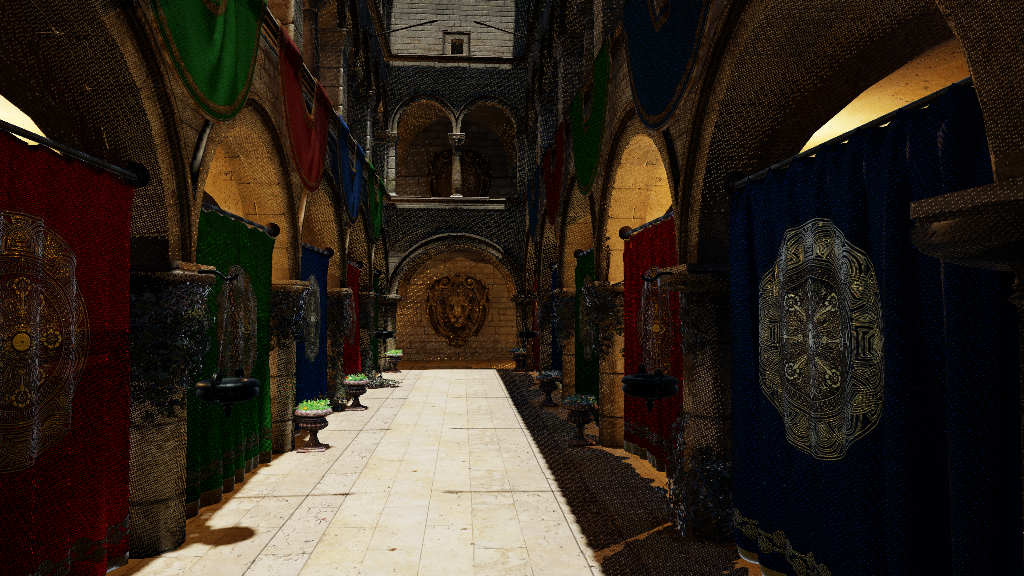
\includegraphics[width=0.48\textwidth]{figures/spp_sweep_1.png}\hfill%
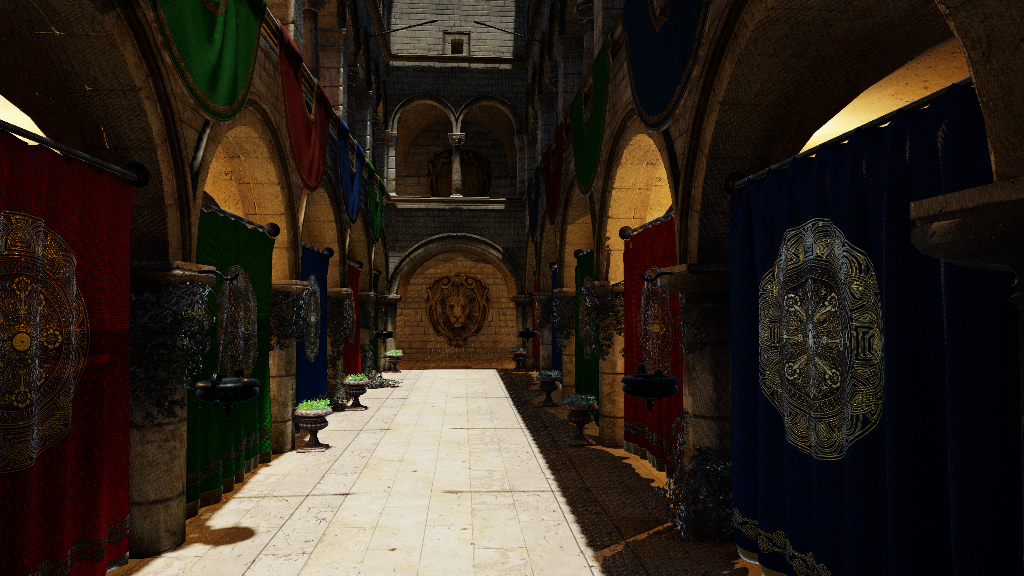
\includegraphics[width=0.48\textwidth]{figures/spp_sweep_8.png}
\caption[Sirovi GI \v{s}um pri jednom i osam zraka]{Uticaj zraka po pikselu na \v{s}um pre uklanjanja \v{s}uma, pre temporalnog razre\v{s}avanja i sa isklju\v{c}enim TAA
(GI; 1 zrak levo, 8 zraka po pikselu desno): vi\v{s}e zraka konvergira ka referenci uz
srazmerno vi\v{s}u cenu (Tabela~\ref{tab:raycount}).}
\label{fig:spp-sweep}
\end{figure}

\section{Polovina naspram pune rezolucije}
\label{sec:halfres}

Pra\'cenje dva hemisferna efekta prikupljanja u polovini rezolucije je najve\'ca pojedina\v{c}na odluka o ceni u
rendereru (Odeljak~\ref{sec:rendergraph}). Pode\v{s}avanje \texttt{render.gi.scale} i \texttt{render.ao.scale} na 1.0 isklju\v{c}uje je, ne menjaju\'ci ni\v{s}ta drugo, pa
se dve konfiguracije razlikuju u ta\v{c}no jednoj promenljivoj.

\begin{table}[tbp]
\caption[Pra\'cenje u polovini naspram pune rezolucije]{Polovina naspram pune rezolucije za GI i AO pra\'cenje (RX 9070 XT). Vreme je ukupno GPU vreme
konfiguracije \texttt{+gi}, a kvalitet je meren sa gledi\v{s}ta atrijuma naspram
konvergirane path-traced reference.}
\label{tab:halfres}
\centering
\input{data/halfres.tex}
\end{table}

Pra\'cenje u punoj rezoluciji ko\v{s}ta \hrDeltaMs{} ms vi\v{s}e po frejmu, pove\'canje od \hrDeltaPct\% na
bud\v{z}et od \hrHalfTotal{} ms, i vra\'ca \hrPsnrGain{} dB PSNR-a: dve konfiguracije su identi\v{c}ne
na drugoj decimali. SSIM i FLIP se pomeraju za 0.0008 i 0.0002, oba daleko unutar rasipanja
izme\dj{}u pokretanja. \v{C}itanje nije \rqt{puna rezolucija je malo bolja}, ve\'c \rqt{merenje ih ne
mo\v{z}e uop\v{s}te da razlikuje}.

Razlog je to \v{s}to je denoiser ograni\v{c}avaju\'ci \v{c}inilac, a ne mre\v{z}a uzoraka. Obe konfiguracije
hrane isti à-trous filter, \v{c}ije jezgro sa zaustavljanjem na ivicama ve\'c zamu\'cuje okolinu \v{s}iru od
faktora dva koji ih razdvaja, pa dodatne uzorke usrednjava upravo onaj filter koji \v{c}ini rezultat u
polovini rezolucije upotrebljivim. Obrazac polovina rezolucije plus bilateralni upsample stoga je
skoro besplatan, a ne kompromis kvaliteta prihva\'cen radi brzine.

Slika~\ref{fig:halfres-buffer} prikazuje sirovu GI iradijansu pod oba pode\v{s}avanja, snimljenu kroz
debug prikaz koji zaobilazi upsample, denoiser i kompoziciju. Bafer u polovini rezolucije nosi
44\% vi\v{s}e visokofrekventne energije po meri hrapavosti iz Odeljka~\ref{sec:raycount} (41.68
naspram 28.91). Ta mera je ponovljiva tamo gde razlika po pikselu nije: drugi
snimak u punoj rezoluciji sa identi\v{c}nim pode\v{s}avanjima daje 28.85, u okviru 0.2\%, a od
prvog se razlikuje za 18.3 nivoa sivog po pikselu samo zato \v{s}to su dva pra\'cenja izvukla razli\v{c}ite slu\v{c}ajne uzorke. Dakle
razlika od 35.4 po pikselu izme\dj{}u bafera u polovini i punoj rezoluciji je samo oko dvostruko ve\'ca od
praga izme\dj{}u pokretanja i nosi malo informacije, dok je razlika u hrapavosti daleko izvan njega. \v{C}etiri
puta vi\v{s}e zraka zaista daje merljivo \v{c}i\v{s}\'ci bafer, iako Tabela~\ref{tab:halfres} pokazuje da
ni\v{s}ta nizvodno od filtera to ne \v{c}uva.

\begin{figure}[tbp]
\centering
\begin{minipage}{0.48\textwidth}\centering
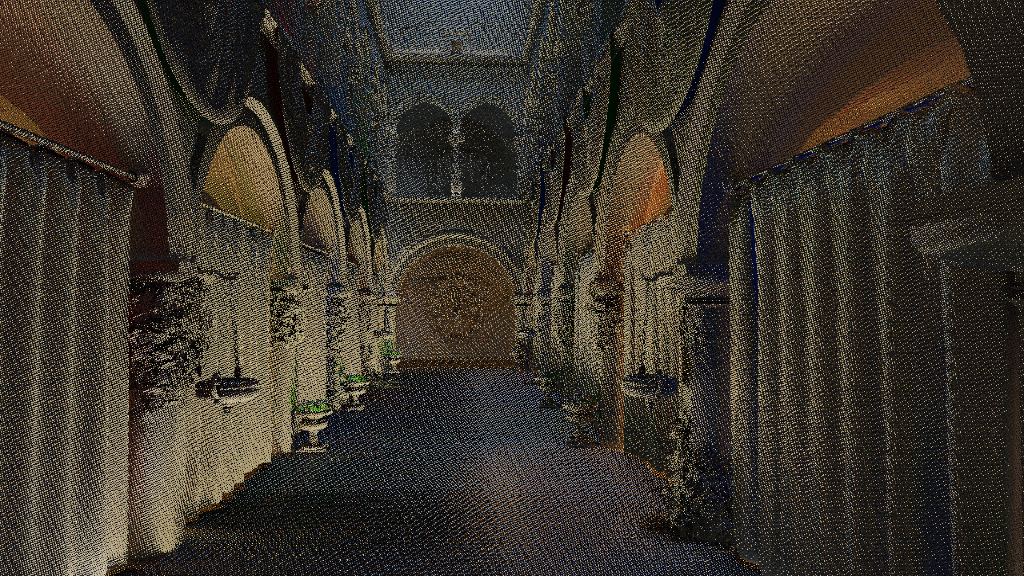
\includegraphics[width=\linewidth]{figures/gi_halfres.png}\\{\small pola (0.5)}
\end{minipage}\hfill
\begin{minipage}{0.48\textwidth}\centering
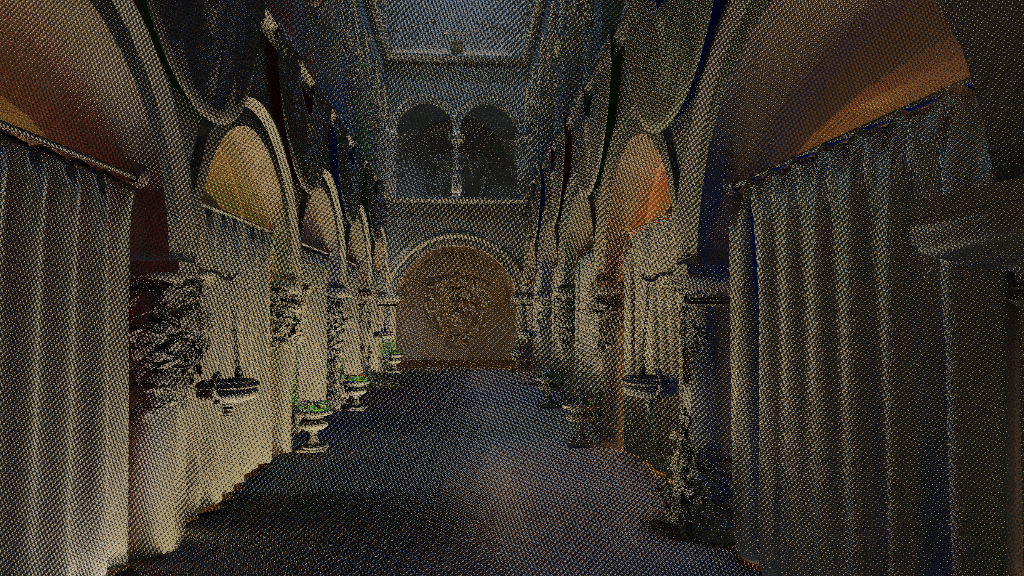
\includegraphics[width=\linewidth]{figures/gi_fullres.png}\\{\small puna (1.0)}
\end{minipage}
\caption[Sirovi GI bafer: polovina naspram pune rezolucije]{Sirovi GI bafer pre upsample-a i
denoisera, pri \texttt{render.gi.scale} 0.5 i 1.0 (\texttt{render.debugview} 6). Puna rezolucija daje
\v{s}iro zrno: 28.91 naspram 41.68 po meri visokofrekventne energije. U kona\v{c}noj slici ta
razlika se ne meri (Tabela~\ref{tab:halfres}).}
\label{fig:halfres-buffer}
\end{figure}

Dva upozorenja ograni\v{c}avaju tu tvrdnju. Vrednosti kvaliteta dolaze sa jednog gledi\v{s}ta, a ne iz prose\v{c}ne
vrednosti tri pogleda kori\v{s}\'cene drugde, a zaklju\v{c}ak je specifi\v{c}an za difuzne signale prikupljanja: kao \v{s}to
Odeljak~\ref{sec:rendergraph} obrazla\v{z}e, isti tretman primenjen na senke ili refleksije
uni\v{s}tio bi ta\v{c}no visokofrekventni detalj zbog kog ti efekti postoje, zbog \v{c}ega se nijedan
ne prati u polovini rezolucije.

\section{Evaluacija denoisera (SVGF)}
\label{sec:denoise-eval}

Sopstveni doprinos SVGF prostornog denoisera izoluje se dr\v{z}anjem temporalne akumulacije konstantnom
(uklju\v{c}ene u oba stanja, stabilizovano preko 90 frejmova) i ocenjivanjem ulaza sa \v{s}umom naspram denoisiranog
rezultata naspram path-traced reference, pri fiksna 2 zraka po pikselu, RX 9070 XT.

\begin{table}[htb]
\centering
\caption[Doprinos SVGF denoisera na mirnom frejmu]{Doprinos SVGF denoisera naspram
path-traced reference (2 zraka/piksel, temporalno razre\v{s}avanje uklju\v{c}eno u oba slu\v{c}aja). Dva reda se razlikuju
za manje od rasipanja ovih metrika izme\dj{}u pokretanja, pa ova tabela pokazuje da filter ne pravi \emph{nikakvu
merljivu razliku} na stabilizovanom mirnom frejmu, a ne da ga pogor\v{s}ava.}
\label{tab:denoise-eval}
\input{data/denoise-eval.tex}
\end{table}

Sa ve\'c aktivnom temporalnom akumulacijom, prostorni SVGF prolaz menja stati\v{c}ke metrike iz
Tabele~\ref{tab:denoise-eval}
(PSNR, SSIM, FLIP) za manje od \v{s}uma merenja, daleko unutar pragova iz
Tabele~\ref{tab:metrics}. Slika~\ref{fig:denoise-compare} pokazuje \v{s}ta ceo lanac rekonstrukcije
radi istom frejmu. Temporalna istorija radi u su\v{s}tini svu
vidljivu konvergenciju na ovom stabilizovanom frejmu, a doprinos samog filtera pokazuje se u temporalnoj
stabilnosti. RMS delta izme\dj{}u frejmova na istom mirnom pogledu (frejm $N$ naspram $N{+}1$ u
stabilnom stanju, proksi treperenja pri statičnoj kameri, a ne kretanje) pada sa \flickerOff{} sa
isklju\v{c}enim denoiserom na \flickerOn{} sa uklju\v{c}enim, smanjenje od \flickerPct\%. Taj proksi je jedini
broj stabilnosti specifi\v{c}an za denoiser ovde, i verovatno potcenjuje filter, jer stati\v{c}na kamera
ne mo\v{z}e da optereti temporalni. Odeljak~\ref{sec:motion} meri stabilnost kako treba pod kretanjem,
ali varira tehniku, a ne filter, pa ograni\v{c}ava ono \v{s}to ceo lanac rekonstrukcije
posti\v{z}e, a ne ono \v{s}to ovaj prolaz doprinosi. Smanjenje treperenja je osetljivo na
jedan detalj protokola: ako se temporalna istorija ne o\v{c}isti pre uzorkovanja, slu\v{c}aju bez filtera
se pripisuje \v{s}um nakupljen dok su se resursi jo\v{s} u\v{c}itavali, \v{s}to napuhuje prividno
smanjenje na blizu 40\%, pa snimci sa tim \v{c}i\v{s}\'cenjem i bez njega nisu uporedivi. GPU cena
denoisera \v{c}ita se iz njegovih sopstvenih timestamp opsega, a ne iz A/B celog frejma: tri
\texttt{GIDenoise} à-trous iteracije ukupno ko\v{s}taju \perfDenoiseAMD{} ms na 9070 XT i
\perfDenoiseNV{} ms na 5070 (Tabela~\ref{tab:pass-cost}), naspram bud\v{z}eta celog frejma blizu devet
milisekundi, a jeftine su delom jer rade u polovini rezolucije. Uklju\v{c}ivanje i isklju\v{c}ivanje denoisera
i oduzimanje ukupnih vrednosti celog frejma daje oko 0.07 ms, \v{s}to ne treba navoditi: manje je od
rasipanja izme\dj{}u pokretanja identi\v{c}ne konfiguracije, pa meri \v{s}um, a ne filter.

Debug prikazi 6 i 7 izoluju filter od svega ostalog na slici, prikazuju\'ci bafer GI iradijanse u polovini
rezolucije kakvog ga trace ostavlja i posle temporalne akumulacije plus à-trous, pre nego \v{s}to se
bilo koji upsample-uje ili kompozituje (Slika~\ref{fig:gi-denoise-ab}). Visokofrekventna energija definisana
u Odeljku~\ref{sec:raycount} pada sa \hfGiRaw{} na \hfGiDenoised{} izme\dj{}u ta dva, oko 96\% od
nje, dok srednji nivo raste jer filter popunjava piksele gde je svaki zrak slu\v{c}ajno
promašio.

Dakle filter skoro potpuno transformi\v{s}e me\dj{}ubafer, a ipak je kona\v{c}na slika
nepromenjena u okviru \v{s}uma merenja. Pipeline nizvodno upija taj posao: bafer se
upsample-uje iz polovine rezolucije, mno\v{z}i albedom povr\v{s}ine, dodaje direktnom osvetljenju koje mu dominira,
pa prolazi kroz temporalno razre\v{s}avanje koje je samo jak niskopropusni filter u vremenu. Pri dva zraka po pikselu sa
ve\'c aktivnom temporalnom akumulacijom, prostorni à-trous je skoro suvi\v{s}an za globalno
osvetljenje i gori nego suvi\v{s}an za refleksije, zbog \v{c}ega se za prvo zadr\v{z}ava na tri iteracije,
a za drugo isklju\v{c}uje, umesto da se primeni uniformno, i govori u prilog tome da se
bud\v{z}et rekonstrukcije prvo tro\v{s}i na temporalnoj, pa tek onda na prostornoj strani.

\paragraph{Isti filter \v{s}teti refleksijama.} Isti à-trous radi na signalu refleksija
i tamo se pokazao neto negativnim, zbog \v{c}ega je sada podrazumevano isklju\v{c}en: njegovo isklju\v{c}ivanje
pobolj\v{s}alo je svaku prostornu metriku odjednom, FLIP 0.1742 naspram 0.1746, PSNR 21.75 naspram 21.70, SSIM
0.6473 naspram 0.6419. To \v{s}to se sve tri pomeraju u istom smeru razlikuje ovo od igranja metrikama,
jer je potpis puko uklanjanja zamu\'cenja to da se FLIP i PSNR pobolj\v{s}avaju dok SSIM pada. Strukturni
razlog je to \v{s}to filter vode normala i dubina povr\v{s}ine koja prima, \v{s}to je ispravno
za difuzno prikupljanje, a pogre\v{s}no za refleksije: reflektovana radijansa zavisi od pogleda, pa su na
ravnoj reflektuju\'coj povr\v{s}ini te vodilje konstantne i jezgro se \v{s}iroko otvara upravo tamo gde reflektovani
detalj \v{z}ivi. Lanac je radio u punoj rezoluciji bez upsample-a posle sebe, pa njegovo uklanjanje izbacuje
lanac prolaza u punoj rezoluciji iz cene refleksija u
Tabeli~\ref{tab:cena}. Jezgro vo\dj eno hrapavo\v{s}\'cu ostaje strukturno ispravno re\v{s}enje, iako sada
mora da pobedi isklju\v{c}eno filtriranje, a ne tri iteracije.

\paragraph{Cena filtera nije ista kod oba proizvo\dj a\v{c}a.} Odmotavanje spoljne petlje à-trous, u\v{c}injeno da bi se
smanjio pritisak na registre \v{s}ejdera (Odeljak~\ref{sec:occupancy}), isplatilo se asimetri\v{c}no: na RTX
5070 je svaki korak postao br\v{z}i, dok je na RX 9070 XT bilo pribli\v{z}no nule na lancima GI i AO u polovini rezolucije
(prva iteracija sporija, poslednja br\v{z}a), a isplatilo se samo na lancima u punoj rezoluciji.
Tabela po prolazima pokazuje ostatak: AMD lanac denoisa je optere\'cen na po\v{c}etku (\texttt{GIDenoise0}
\perfGiDenoiseFirstAMD{} ms pada na \perfGiDenoiseLastAMD{} ms pri \texttt{GIDenoise2}), dok se NVIDIA obr\'ce (\perfGiDenoiseFirstNV{} ms raste na
\perfGiDenoiseLastNV{} ms). To je ista asimetrija zavisna od rezolucije izolovana u Odeljku~\ref{sec:cena}, vi\dj ena
s druge strane, a lokalnost naspram zauzetosti pri u\v{z}em koraku je o\v{c}igledna poluga. Kao
tamo, timestampovi je ne mogu razdvojiti od alternativa, a za to su potrebni brojači memorije
koje ovaj rad ne meri. Ono \v{s}to brojevi utvr\dj uju je prakti\v{c}na poenta: optimizacija \v{s}ejdera
opravdana brojem registara nije automatski dobitak i mora se meriti po proizvo\dj a\v{c}u kao sve ostalo u ovoj glavi.

\begin{figure}[tbp]
\centering
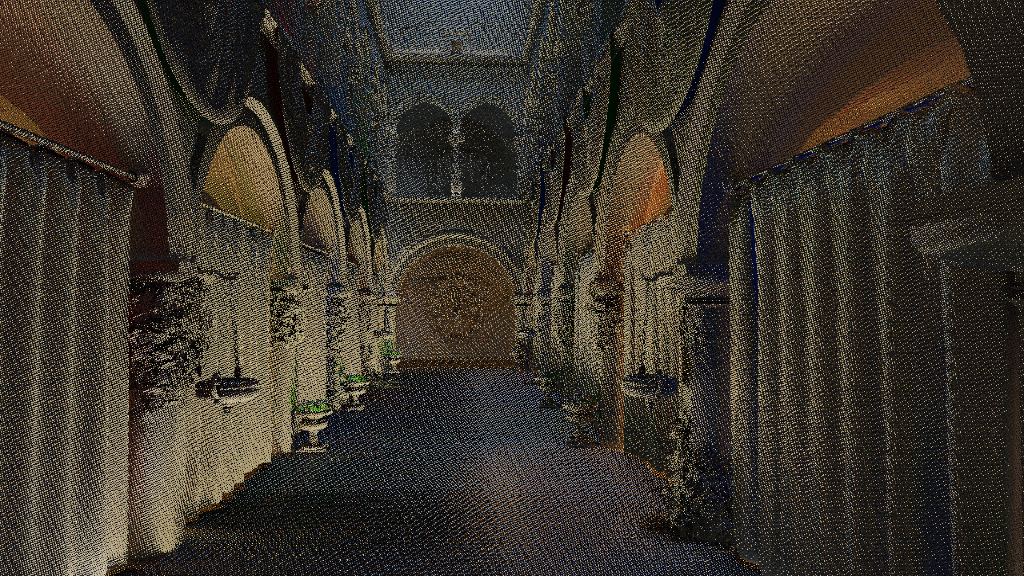
\includegraphics[width=0.48\textwidth]{figures/dbg_gi_raw.png}\hfill%
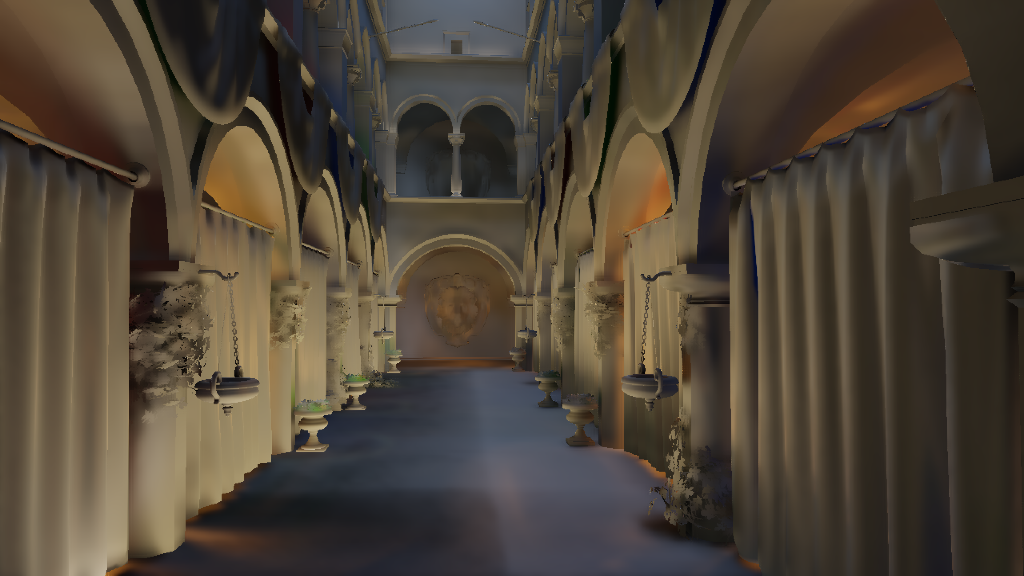
\includegraphics[width=0.48\textwidth]{figures/dbg_gi_denoised.png}
\caption[GI iradijansa pre i posle rekonstrukcije]{GI iradijansa u polovini rezolucije pre (levo) i posle (desno) temporalne akumulacije i
a-trous filtera, pre upsample-a i kompozicije (\texttt{render.debugview} 6 i 7). Levo je
zrnasti signal od jednog zraka, desno isti bafer posle rekonstrukcije.}
\label{fig:gi-denoise-ab}
\end{figure}

\begin{figure}[tbp]
\centering
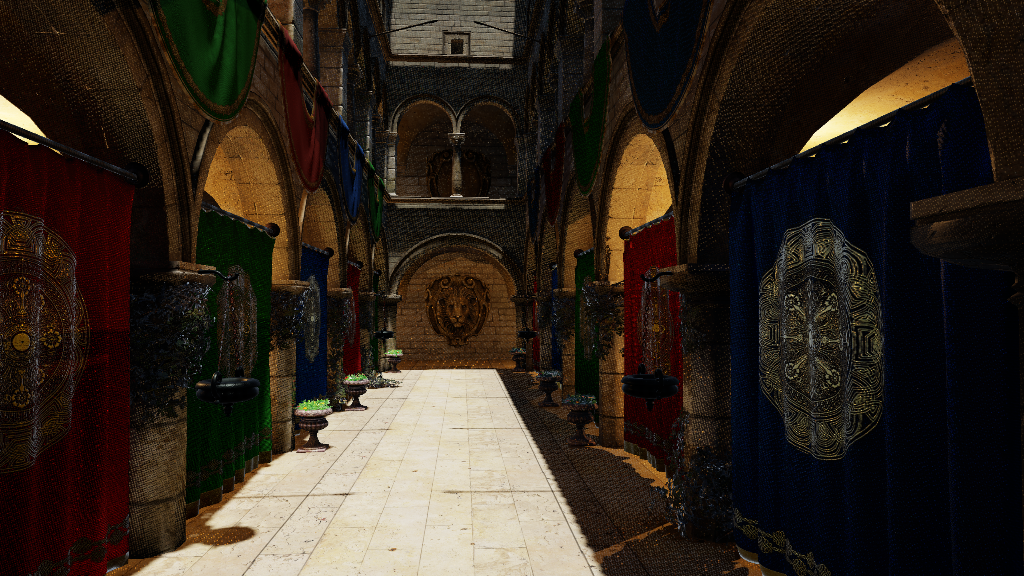
\includegraphics[width=0.62\textwidth]{figures/denoise_compare_noisy.png}

\vspace{5pt}

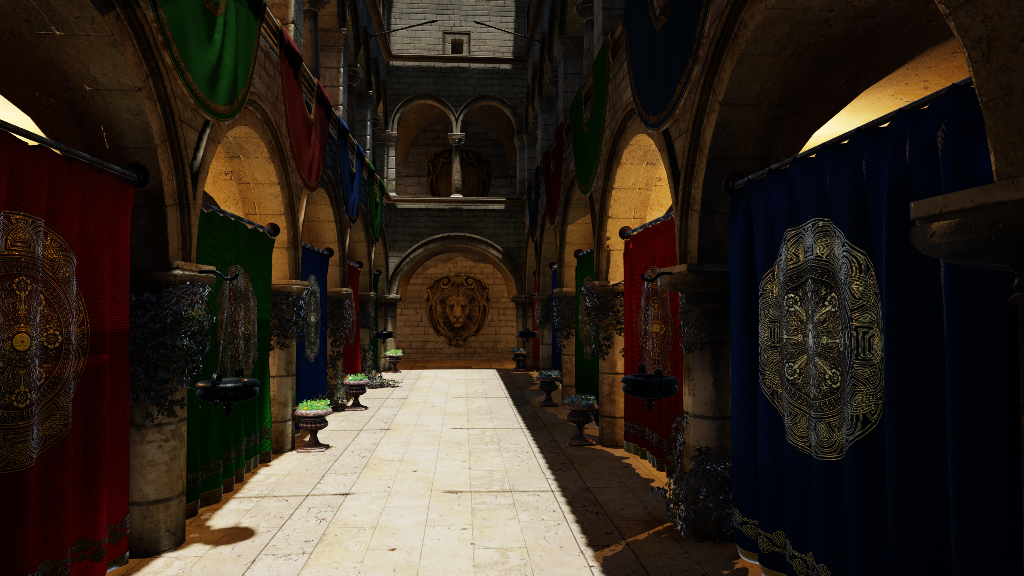
\includegraphics[width=0.62\textwidth]{figures/denoise_compare_denoised.png}

\vspace{5pt}

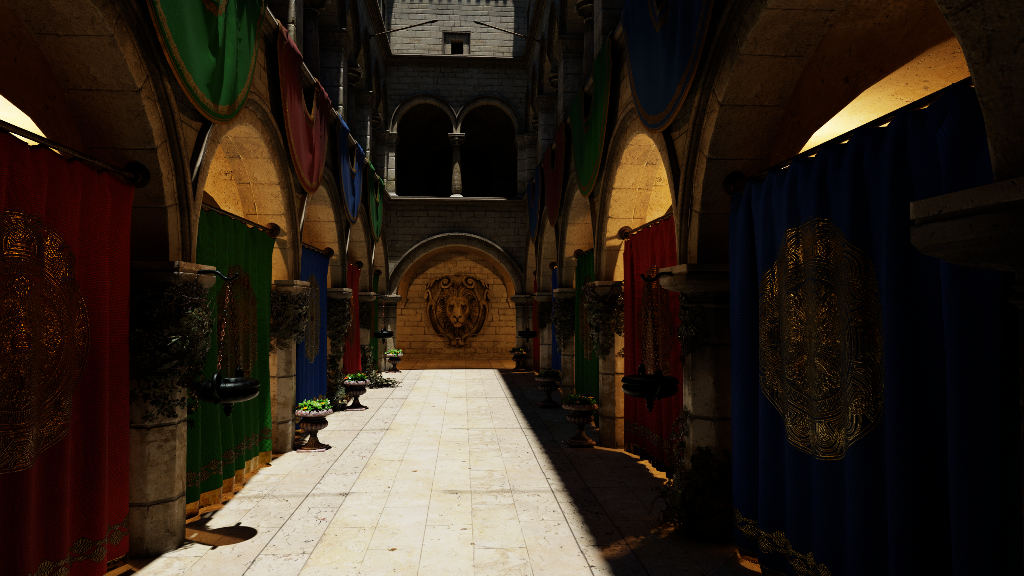
\includegraphics[width=0.62\textwidth]{figures/denoise_compare_reference.png}
\caption[Sirovi signal, rekonstrukcija i referenca]{Rekonstrukcija pri 2 zraka po pikselu: sirovi signal sa isklju\v{c}enim denoiserom, temporalnim razre\v{s}avanjem i TAA
(gore), pun rezultat u realnom vremenu sa sva tri uklju\v{c}ena (sredina) i path-traced
referenca (dole). Razlika od gornje do srednje je doprinos cele rekonstrukcije, dok je
sopstveni doprinos denoisera izolovan metrikama u tekstu, gde se pokazuje prvenstveno u temporalnoj
stabilnosti.}
\label{fig:denoise-compare}
\end{figure}

\section{Poređenje sa postoje\'cim re\v{s}enjima}
\label{sec:poredjenje}

Engine implementira rasterske screen-space osnovne linije za ambijentalnu okluziju i refleksije (SSAO, SSR;
Odeljak~\ref{sec:efekti}), pa je poređenje sa re\v{s}enjima prikazanim u
Glavi~\ref{ch:pregled} A/B na istoj sceni sa istom kamerom, koje izla\v{z}e slu\v{c}ajeve s kojima screen-space metoda
strukturno ne mo\v{z}e da izađe na kraj: okludere i reflektore van ekrana i disokluziju
(Slika~\ref{fig:rt-vs-ss}). Pozicioniranje naspram produkcijskih sistema (Lumen, RTXGI, ReSTIR) je
kvalitativno: doprinos je integrisana, izmerena, otvoreno licencirana implementacija sa ray query-jem,
a ne sistem koji nadma produkcijsko re\v{s}enje za globalno osvetljenje.

\begin{table}[tbp]
\caption[Kvalitet svake tehnike naspram reference]{Kvalitet svake tehnike naspram path-traced reference (usrednjeno preko tri gledi\v{s}ta:
atrijum, pod, galerija; RX 9070 XT). Ni\v{z}i FLIP i vi\v{s}i PSNR/SSIM su bolji.}
\label{tab:quality}
\centering
\input{data/quality.tex}
\end{table}

\begin{figure}[tbp]
\centering
\begin{tikzpicture}
\begin{axis}[width=0.88\textwidth, height=6.2cm,
  ylabel={FLIP $\downarrow$}, ymin=0, ymax=0.58,
  xtick={0,...,9},
  xticklabels={raster,SSAO,RT AO,SSR,RT refl.,RT shad.,RT shad. stoch.,SSGI,RT GI,all-RT},
  xticklabel style={font=\small, rotate=25, anchor=north east},
  tick label style={font=\small}, label style={font=\small},
  grid=major, grid style={black!12}, enlarge x limits=0.08]
\addplot[only marks, mark=*, mark size=2pt, black,
  error bars/.cd, y dir=both, y explicit]
  table[col sep=tab, x=i, y=flip, y error plus expr=\thisrow{hi}-\thisrow{flip},
        y error minus expr=\thisrow{flip}-\thisrow{lo}] {data/quality-spread.dat};
\end{axis}
\end{tikzpicture}
\caption[FLIP po tehnici sa rasipanjem preko gledi\v{s}ta]{Isti podaci kao
Tabela~\ref{tab:quality}, sa opsegom preko tri gledi\v{s}ta umesto samog proseka.
Trake su varijacija sadr\v{z}aja, a ne gre\v{s}ka merenja: govore da kadriranje pomera ocenu vi\v{s}e nego
ve\'cina ovih tehnika, pa dve preklopljene trake nisu dve nerazlu\v{c}ive
tehnike. Ponovljivost je otprilike 0.0024 FLIP, daleko u\v{z}a od bilo koje ovde nacrtane trake, pa su
razlike izme\dj{}u grupisanih ta\v{c}aka stvarne \v{c}ak i kad im se opsezi skoro potpuno preklapaju.
Rasipanje je i samo deo rezultata: raster ide od \qRasterFlipLo{} do \qRasterFlipHi{}
zavisno od kadriranja, dok RT GI ostaje u \qRtGiFlipLo{}--\qRtGiFlipHi{}. Tehnike koje
re\v{s}avaju indirektno osvetljenje su ta\v{c}nije u proseku i ujedna\v{c}enije preko scene, \v{s}to
sam prosek ne pokazuje.}
\label{fig:quality-spread}
\end{figure}

Naspram path-traced reference (Tabela~\ref{tab:quality}, sa rasipanjem po gledi\v{s}tu na
Slici~\ref{fig:quality-spread}) globalno osvetljenje je dominantna
poluga kvaliteta: sam RT GI podi\v{z}e
PSNR sa \qRasterPsnr{} (raster) na \qRtGiPsnr{} i smanjuje FLIP za vi\v{s}e od dve tre\'cine, a uklju\v{c}ivanje
svih efekata dosti\v{z}e FLIP \qAllRtFlip{}, PSNR \qAllRtPsnr{}, SSIM \qAllRtSsim{}, daleko najbli\v{z}e
referenci.

\paragraph{Gde je dobitak i \v{s}ta ekspozicija ima s tim.} Scena je tamna:
\exDarkShare\% piksela reference je ispod desetine pune luminanse, sa medijanom od
\exMedianLuma{}, jer su sunce i \v{c}etiri baklje jedina uklju\v{c}ena svetla, a tri
definisana reflektora kroz prozore Sponze su isklju\v{c}ena. To name\'ce prigovor da je dobitak dva renderovanja
koja se sla\v{z}u oko tame. Referenca je path trace iste scene sa istom ekspozicijom, pa
samo poređenje nije zahva\'ceno, ali VELI\v{C}INA dobitka jeste. Ponovno ocenjivanje gledi\v{s}ta atrijuma
na sve svetlijim podskupovima reference (maskiranje na referenci, nikad na tehnici,
\v{s}to bi dozvolilo tehnici da bira sebi povoljne piksele) menja dobitak od rastera do all-RT
sa \exLiftAll{} dB preko celog frejma na \exLiftLit{} dB preko najsvetlijih \exLitShare\%. Raster je
ono \v{s}to se pomera: ide sa \exRasterAll{} dB na \exRasterLit{} dB kako se tamni pikseli odbacuju, dok
se rezultat sa pra\'cenjem zraka jedva menja. Rasterizacija je skoro ta\v{c}na svuda gde svetlost stiže
direktno i zaostaje svuda gde ne stiže, pa se prednost koncentri\v{s}e u indirektno osvetljenom
delu frejma. Tu je mesto gde ova \v{c}etiri efekta treba da budu bitna, a koncentracija je
o\v{c}ekivani potpis, a ne artefakt, ali to zna\v{c}i da je naslovni iznos u decibelima
svojstvo ove ekspozicije koliko i tehnika, a svetlija scena bi prijavila manji.

Na ovim
metrikama celog frejma screen-space i ray-traced AO i refleksije su skoro izjedna\v{c}eni (SSAO naspram RT AO,
i SSR naspram RT refleksija, razlikuju se za manje od 0.01 u FLIP-u), jer su doprinosi okluzije i refleksije
mali na nivou celog frejma. Snimljen kroz debug prikaz koji izoluje samo
AO \v{c}lan, gledi\v{s}te atrijuma ima medijanu AO
od 255 od 255, tj. nikakvu okluziju, a samo 14.1\% (SSAO) i 17.6\% (RT AO) piksela pada
ispod 240. Efekat koji ostavlja pet \v{s}estina frejma netaknutim ne mo\v{z}e mnogo da pomeri prosek celog frejma,
kako god da se ra\v{c}una. Prednost pra\'cenja zraka je ta\v{c}nost van ekrana, koju prosek celog frejma
ne izoluje. Slike~\ref{fig:ssvsrt-ao} i~\ref{fig:ssvsrt-refl} je izoluju
za AO i za refleksije prikazuju\'ci same te bafere umesto kompozitovanog frejma.

\v{C}itana naspram cena, tri efekta se \v{c}isto razdvajaju, a razdvajanje je u dobitku,
a ne u ceni (Slika~\ref{fig:tradeoff}). Svaki od njih zaista pobolj\v{s}ava frejm u odnosu na \v{c}istu
rasterizaciju, za 0.0205 FLIP kod RT AO i 0.0122 kod RT refleksija naspram praga merenja od
0.0024, pa nijedan ne radi ni\v{s}ta. Ali pitanje s kojim se renderer zaista suo\v{c}ava je da li
ray-traced verzija zaslu\v{z}uje svoj multiplikator nad screen-space verzijom, a tu se odgovori razlikuju za
red veli\v{c}ine dok se cene ne razlikuju.

Na metrikama celog frejma prednost pra\'cenja zraka je stoga odlu\v{c}uju\'ca za globalno osvetljenje,
marginalna za refleksije i nerazre\v{s}ena za ambijentalnu okluziju. Taj redosled je svojstvo
metrike koliko i tehnika, iz gore datog razloga, a izolovani baferi ispod pokazuju
razlike koje kompozitovani prosek ne mo\v{z}e. Ali pravac vredi navesti jasno, umesto da se
prepusti \v{c}itaocu: ova evaluacija pokazuje vrednost pra\'cenja zraka za indirektno difuzno
osvetljenje, a ne pokazuje je za okluziju.

\begin{figure}[tbp]
\centering
\begin{tikzpicture}
% Log y: the three gains span 73x (0.0027 to 0.1978), so on a linear axis two of the three sit on the
% x-axis, indistinguishable from each other and from the measurement floor. The floor is the point of
% the figure, since AO clears it by 12% and reflections by 2.9x, and only a log axis shows that.
\begin{axis}[width=0.82\textwidth, height=6.4cm,
  xlabel={cena pra\'cenja zraka, kao umno\v{z}ak screen-space metode},
  ylabel={FLIP dobijen preko nje}, ymode=log,
  ymin=0.0018, ymax=0.42, xmin=1.35, xmax=3.7,
  ytick={0.002,0.005,0.01,0.02,0.05,0.1,0.2},
  yticklabels={0.002,0.005,0.01,0.02,0.05,0.10,0.20},
  grid=major, grid style={black!12},
  tick label style={font=\small}, label style={font=\small}]
\draw[dashed, black!55] (axis cs:1.35,0.0024) -- (axis cs:3.7,0.0024);
\node[font=\scriptsize, black!55, anchor=south east] at (axis cs:3.68,0.0024)
  {prag merenja};
% Segments, markers and label positions all come from data/tradeoff-seg.dat and data/tradeoff.dat
% (tools/gen_perf_plots.py), so they cannot drift from the ladder numbers.
\addplot[black!55, line width=1.1pt] table[col sep=tab, x=mult, y=flipGain] {data/tradeoff-seg.dat};
\addplot[only marks, mark=*, mark size=2.2pt, black] table[col sep=tab, x=mult, y=flipGain] {data/tradeoff-seg.dat};
\addplot[only marks, mark=none, font=\small, nodes near coords, point meta=explicit symbolic,
  every node near coord/.style={anchor=south, yshift=4pt}]
  table[col sep=tab, x=mid, y=flipGain, meta=effect] {data/tradeoff.dat};
\end{axis}
\end{tikzpicture}
\caption[\v{S}ta pra\'cenje zraka ko\v{s}ta naspram \v{s}ta vra\'ca]{\v{S}ta pra\'cenje zraka ko\v{s}ta naspram \v{s}ta
vra\'ca, po efektu. Svaki segment obuhvata umno\v{s}ke cene dva adaptera pri dobitku
kvaliteta tog efekta, koji je meren samo na RX 9070 XT, a isprekidana linija je prag merenja iz
Odeljka~\ref{sec:metodologija}. Cene su sve sli\v{c}ne, izme\dj{}u \perfSsFactorMin{} i \perfSsFactorMax{} puta screen-space
metode, a dobici nisu: globalno osvetljenje je za red veli\v{c}ine iznad druga dva,
a ambijentalna okluzija pada na prag. Obe ose se ra\v{c}unaju
unutar jednog para screen-space/ray-traced, odnos i razlika, pa nijedna ne zavisi od toga na kojoj
konfiguraciji par le\v{z}i i razli\v{c}ite osnovne linije dva gejta ne moraju da se sla\v{z}u.}
\label{fig:tradeoff}
\end{figure}

\begin{figure}[tbp]
\centering
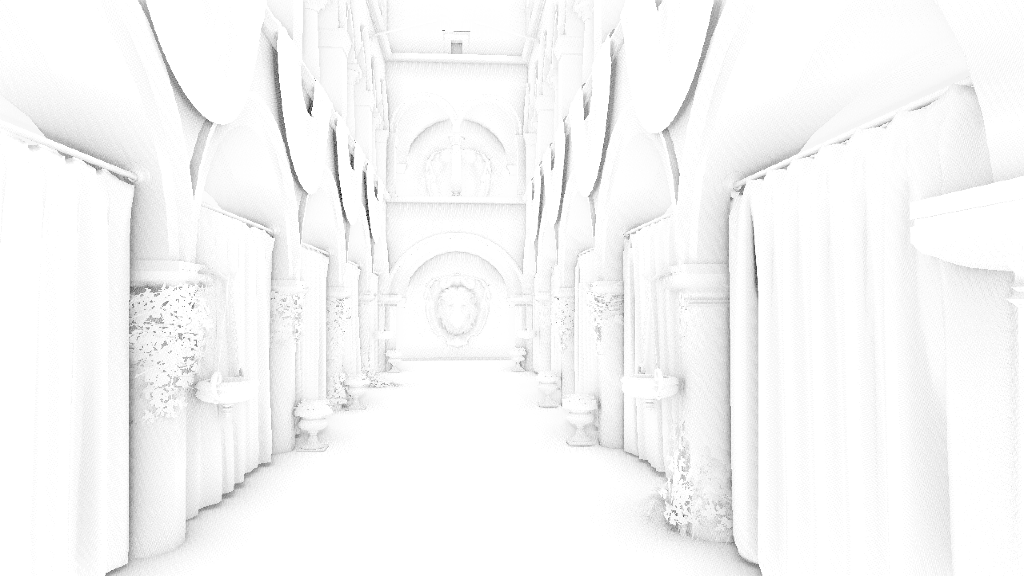
\includegraphics[width=0.485\textwidth]{figures/ssvsrt_ssao.png}\hfill
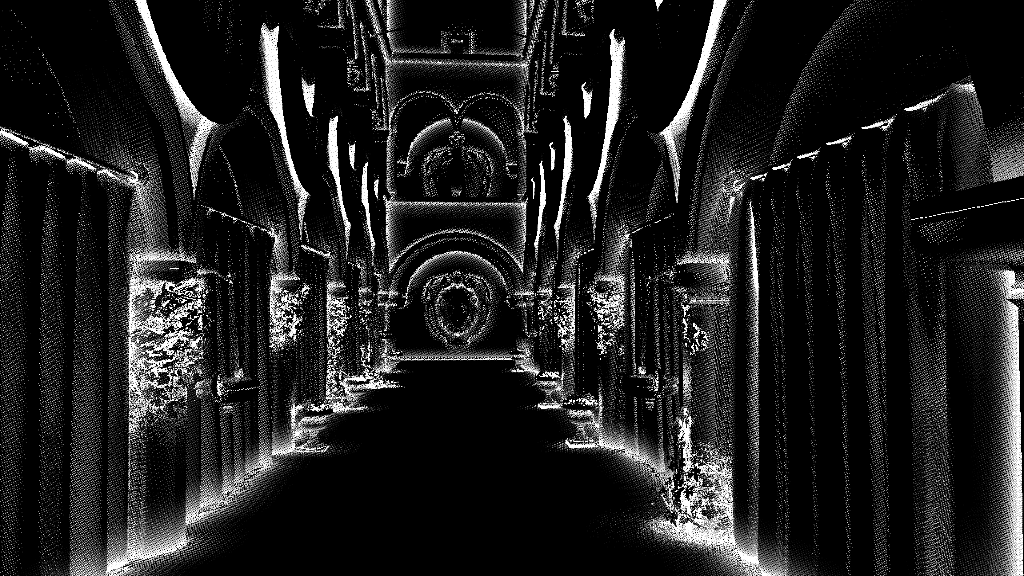
\includegraphics[width=0.485\textwidth]{figures/ssvsrt_rtao.png}
\caption[Screen-space naspram ray-traced ambijentalne okluzije]{Izolovani \v{c}lan okluzije sa gledi\v{s}ta
atrijuma, SSAO (levo) naspram ray-traced AO (desno). Oba panela prikazuju $1-\mathrm{AO}$ sa pojačanjem
4, ista transformacija na obe strane, pa je svetlo okludirano i skoro beli sirovi baferi postaju
\v{c}itljivi. SSAO razre\v{s}ava samo tanak obod gde se dve povr\v{s}ine sastaju u baferu dubine, \v{s}to je sve \v{s}to
mo\v{z}e da vidi, dok pra\'ceni \v{c}lan daje zavesama, svodovima i li\v{s}\'cu okluziju sa telom,
jer okludiraju\'ca geometrija ne mora biti na ekranu. \v{C}itati strukturno, a ne po pikselu: sirovi
stohasti\v{c}ki bafer se ne reprodukuje bit po bit, a dva snimka jedne konfiguracije razlikuju se za
prosek od 3.8 od 255 naspram 8.8 izme\dj{}u tehnika.}
\label{fig:ssvsrt-ao}
\end{figure} Dva producenta senki su tako\dj e skoro izjedna\v{c}ena ovde, \qRtShadowFlip{} za inline putanju naspram
\qMegalightsFlip{} za stohasti\v{c}ku, \v{s}to uti\v{c}e na to kako treba \v{c}itati Odeljak~\ref{sec:analiza-shadow-strategy}:
strategije se u terminima slike ne razlikuju statisti\v{c}ki, pa je inverzija proizvo\dj a\v{c}a
prona\dj ena tamo \v{c}ist rezultat cene, a ne kompromis kvaliteta.
Screen-space GI le\v{z}i izme\dj{}u ta dva nivoa: njegov FLIP (\qSsgiFlip{}) je znatno bolji od
AO/refleksijskih parova, ali daleko od RT GI (\qRtGiFlip{}), u skladu sa tim da SSGI prikuplja odbijenu
svetlost samo iz geometrije na ekranu, dok RT GI dopire i do povr\v{s}ina van ekrana i iza kamere.

\begin{figure}[tbp]
\centering
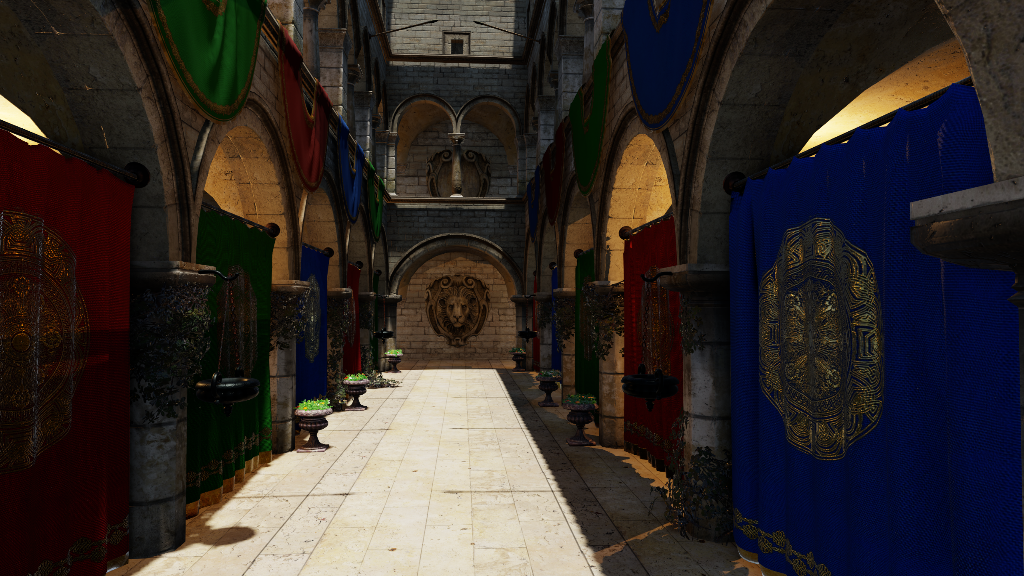
\includegraphics[width=0.48\textwidth]{figures/ss_all.png}\hfill%
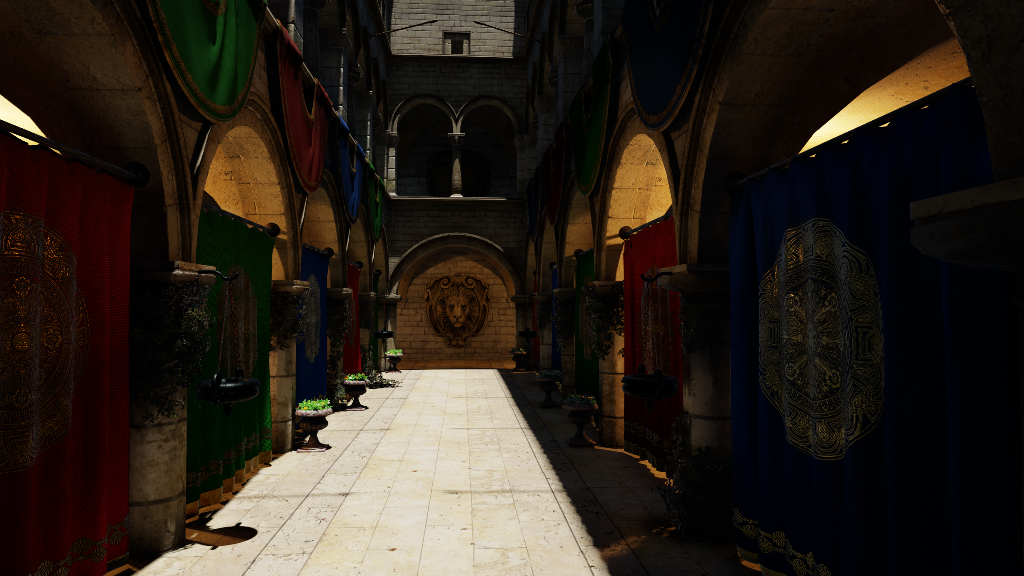
\includegraphics[width=0.48\textwidth]{figures/rt_all.png}
\caption[Screen-space naspram ray-traced konfiguracije]{Ista scena i kamera u dve kompletne
konfiguracije: screen-space (levo: mapa senki, SSAO, SSR, SSGI) naspram ray-traced (desno: pra\'cene
senke, RTAO, RT refleksije, RT GI). Senke prate ostatak jer screen-space nema parnjaka
pra\'cenoj senci, pa je mapa ono \v{s}to ta porodica zaista koristi. To je ista podela koju koristi red
\rqt{all-RT} Tabele~\ref{tab:quality}. Screen-space varijanta je svetlija jer ne
mo\v{z}e da oduzme svetlost koja stiže iz geometrije van ekrana.}
\label{fig:rt-vs-ss}
\end{figure}

\begin{figure}[tbp]
\centering
\begin{minipage}{0.48\textwidth}\centering
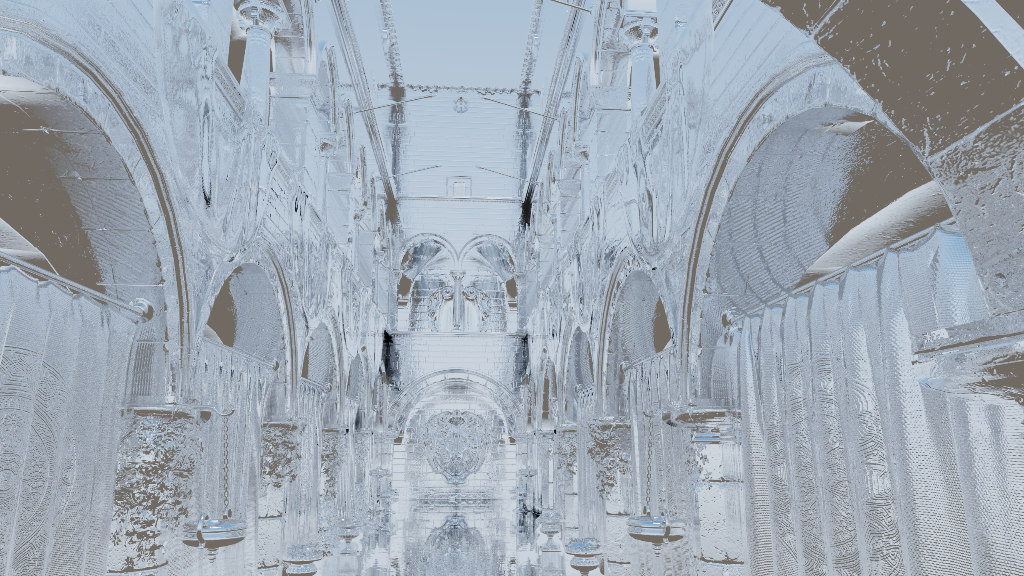
\includegraphics[width=\linewidth]{figures/ssvsrt_ssr.png}\\{\small SSR}
\end{minipage}\hfill
\begin{minipage}{0.48\textwidth}\centering
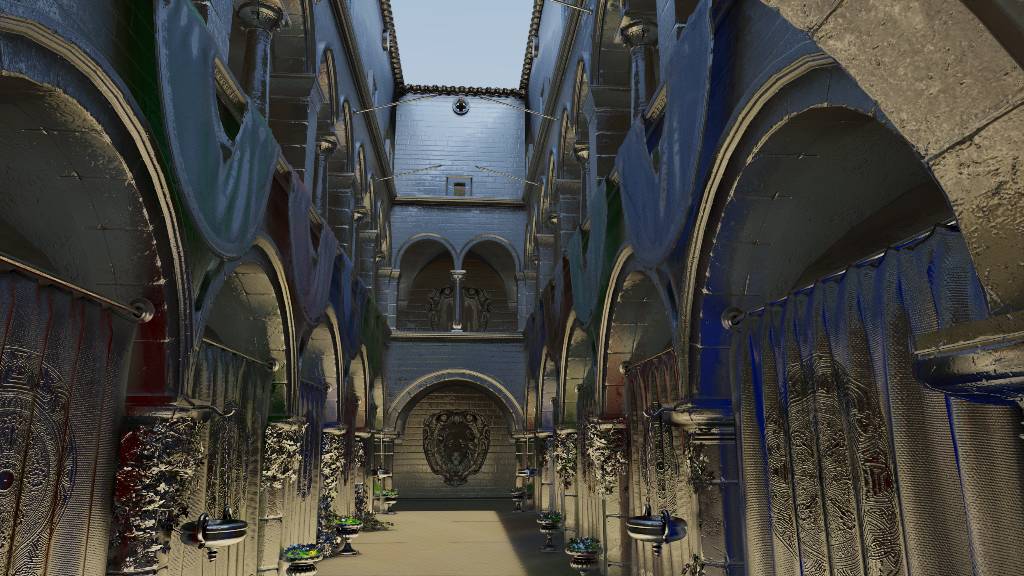
\includegraphics[width=\linewidth]{figures/ssvsrt_rtrefl.png}\\{\small RT refleksije}
\end{minipage}
\caption[Sirovi bafer refleksija: SSR naspram RT]{Sirovi bafer refleksija (\texttt{render.debugview}
3), isto gledi\v{s}te i iste podrazumevane vrednosti. SSR i RT pi\v{s}u u isti bafer, pa je izvor
refleksije jedina promenljiva. Kad marš kroz bafer dubine ne na\dj e ni\v{s}ta, SSR se vra\'ca na prefiltriranu
mapu okoline: 9.0\% piksela je zbog toga skoro belo, naspram 0.0\% desno, a
srednja vrednost bafera je 169.4 naspram 65.99. U kompozitovanom frejmu ta razlika se gubi pod direktnim
osvetljenjem, zbog \v{c}ega dve tehnike imaju skoro isti FLIP.}
\label{fig:ssvsrt-refl}
\end{figure}

\section{Stabilnost pod kretanjem}
\label{sec:motion}

Svaka vrednost kvaliteta do sada dolazi sa stati\v{c}ke kamere, za \v{s}ta je Odeljak~\ref{sec:denoise-eval} utvrdio da
sakriva ve\'cinu onoga \v{s}to prostorni denoiser radi: smanjuje treperenje izme\dj{}u frejmova za \flickerPct\%, a
stati\v{c}ke metrike pomera za manje od \v{s}uma merenja, argument iznet tamo samo preko proksija. Ovaj
odeljak pomera kameru.

Menja i scenu. Stati\v{c}ki gejtovi rade na \texttt{Sponza.world}, koja miruje, pa pokretna
kamera tamo ispituje reprojekciju, ali nikad disokluziju od pokretnog objekta. Ovaj odeljak koristi
\texttt{Sponza-Motion.world} (Slika~\ref{fig:sponza-motion}), isti enterijer sa \v{c}etiri objekta
koji se rotiraju u visini o\v{c}iju izme\dj{}u rute kamere i kolonade, \v{s}to stavlja pokretne
okludere ispred pokretne geometrije. Dve scene su namerno odvojene: animiranje objekata
u \texttt{Sponza.world} poni\v{s}tilo bi svaku commitovanu osnovnu liniju kvaliteta i performansi izmerenu
na njoj.

\begin{figure}[tbp]
\centering
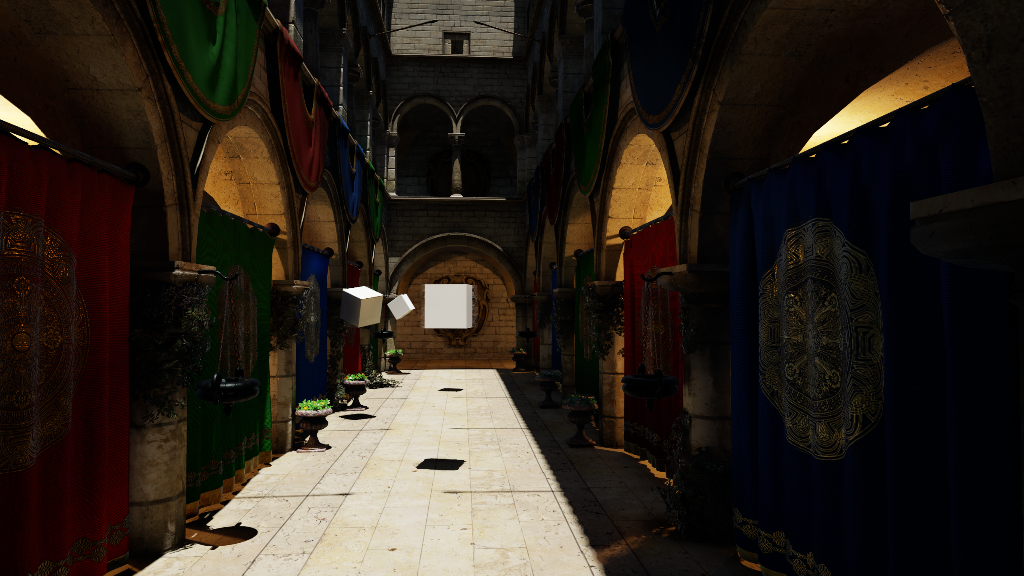
\includegraphics[width=0.92\textwidth]{figures/sponza_motion.png}
\caption[Scena kori\v{s}\'cena za merenja kretanja]{\texttt{Sponza-Motion.world}: test scena
sa \v{c}etiri rotiraju\'ca objekta dodata u visini o\v{c}iju du\v{z} glavnog broda, ovde vidljiva kao bledi kubovi i
senke koje bacaju na pod. Postoje da bi se kretali objekti, a ne samo kamera:
filter sa reprojekcijom mo\v{z}e da prati stati\v{c}nu scenu pod kretanjem kamere samo preko dubine, dok
okluder koji se nezavisno kre\'ce prisiljava filter da odbaci istoriju.}
\label{fig:sponza-motion}
\end{figure}

Prelet fiksne rute, snimanje frejmova du\v{z} nje i ocenjivanje svakog naspram konvergiranog path trace-a
istog trenutka je protokol koji je BMFR uspostavio za animirane sekvence
\cite{koskela2019bmfr}. On proizvodi upozorenje o metodi pre ikakve \v{c}injenice o rendereru: preko
jedanaest tehnika, FLIP po frejmu meren na ovaj na\v{c}in korelira sa stati\v{c}kim FLIP-om iz
Odeljka~\ref{sec:poredjenje} sa $r = +0.99$, skoro isto merenje uzeto dvaput. Konvergirani
path trace po frejmu je niz nezavisnih mirnih slika bez temporalne strukture,
jer ni\v{s}ta u njegovoj konstrukciji ne povezuje jedan frejm sa slede\'cim, pa gre\v{s}ka merena naspram njega nema
temporalnu komponentu koju bi nosila koliko god se kamera pomerala. Mana je u tom eksperimentalnom dizajnu,
a ne u implementaciji, i to je poznato mešanje: k-DOP Clipping
\cite{ikkala2024kdop} otvoreno navodi da supersamplirana referenca uvodi konstantnu gre\v{s}ku
poredi\'ci i op\v{s}ti kvalitet temporalnog antialiasinga sa supersamplingom. Kanonski radovi o denoiserima
to izbegavaju prijavljuju\'ci ta\v{c}nost naspram reference i temporalno pona\v{s}anje odvojeno,
potonje merom bez reference.

Dve veli\v{c}ine u pokretnom snimku nose informaciju koju stati\v{c}ki gejt ne mo\v{z}e. Prva poredi
koliko se tehnika menja izme\dj{}u uzastopnih frejmova naspram toga koliko se \emph{referenca}
menja u istom intervalu, pa se kretanje svojstveno sceni oduzima i ostaje samo vi\v{s}ak
nestabilnosti. Oduzimanje je bitno: na ovoj ruti se sama referenca pomera za FLIP od oko
0.09 izme\dj{}u susednih frejmova, \v{s}to bi naivna razlika frejmova prijavila kao nestabilnost. Rangirane po
njoj (Tabela~\ref{tab:motion}), tehnike se poredaju ta\v{c}no kako je proksi treperenja predvideo,
potpuno rekonstruisane konfiguracije najstabilnije, a \v{c}ista rasterizacija najmanje, \v{s}to je
zaklju\v{c}ak Odeljka~\ref{sec:denoise-eval} dostignut pod kretanjem umesto preko proksija: prostorni
filter kupuje stabilnost, a ne stati\v{c}ku vernost. Dve temporalne metrike se korisno ne sla\v{z}u:
\texttt{rtgi} ima najbolji tFLIP dok \texttt{all-rt} ima najbolji JOD, jer tFLIP izoluje
samo temporalni vi\v{s}ak, a ColorVideoVDP je prostorno-temporalan i \texttt{all-rt} je daleko ta\v{c}niji
prostorno.

\begin{table}[tbp]
\caption[Stabilnost pod kretanjem po tehnici]{Stabilnost pod kretanjem, usrednjena preko \v{c}etiri
ta\v{c}ke sonde rute (RX 9070 XT), rangirano po FLIP-u. tFLIP meri koliko se tehnika menja izme\dj{}u
susednih frejmova preko onoga koliko se sama referenca menja, \v{s}to je konstrukcija tLP iz TecoGAN-a
\cite{chu2020tecogan} sa FLIP-om umesto LPIPS-a, a kašnjenje je pokretni frejm
naspram sopstvenog konvergiranog mirnog frejma u istoj pozi. JOD je ColorVideoVDP
\cite{mantiuk2024cvvdp}, jedina mera ovde koja direktno modeluje temporalnu osetljivost na kontrast.}
\label{tab:motion}
\centering
\input{data/motion.tex}
\end{table}

Druga je kašnjenje: pokretni frejm ocenjen naspram renderer-ovog sopstvenog konvergiranog mirnog frejma u istoj
pozi, \v{s}to meri koliko rekonstrukcija zaostaje za kamerom, i \v{c}ita se du\v{z} rute u
Tabeli~\ref{tab:motion-probes} za dva kraja rang-liste. Obrtanje brzine je najskuplje
kretanje, i to ne zbog brzine, jer ruta dr\v{z}i translaciju u su\v{s}tini konstantnom: posebno kod obrtanja je to
\v{s}to vektor brzine menja znak, dokumentovan patolo\v{s}ki slu\v{c}aj za odbacivanje istorije.
Parkirana sonda je za red veli\v{c}ine ispod pokretnih i slu\v{z}i kao
kontrola koja ih \v{c}ini \v{c}itljivim.

\begin{table}[tbp]
\caption[Stabilnost i kašnjenje po sondi rute]{Iste dve temporalne mere razlo\v{z}ene po ta\v{c}ki sonde,
za krajeve rang-liste. Vrednosti se ne porede preko kolona: svaka sonda gleda razli\v{c}it
sadr\v{z}aj, pa je razlika izme\dj{}u njih uglavnom razlika u onome \v{s}to je na ekranu.}
\label{tab:motion-probes}
\centering
\input{data/motion-probes.tex}
\end{table}

Tri upozorenja idu uz ove brojeve. Ne smeju se porediti preko sondi kao da su sonde
jednako te\v{s}ke, jer svaka gleda drugi sadr\v{z}aj scene: me\dj{}u tri pokretne sonde \v{c}ista
rasterizacija ima svoj \emph{najbolji} FLIP po frejmu na sondi obrtanja, dok tamo pokazuje najgore kašnjenje. Mera kašnjenja je
renderer naspram sopstvenog mirnog frejma, pa se mo\v{z}e svesti na nulu degradiranjem mirnog frejma i nikad se ne sme
koristiti kao cilj optimizacije. A njena apsolutna skala zavisi od protokola snimanja, koji je
ispravljen tokom ovog rada, pa se smeju navoditi samo vrednosti iz trenutnih osnovnih linija i nikad mešati
sa ranijim.

\paragraph{Mere stabilnosti nagra\dj uju zamu\'cenje, a tFLIP nije izuzet.} Svaka mera koja ocenjuje rezultat
po tome koliko se malo menja izme\dj{}u uzastopnih frejmova daje prednost onom koji je izglađen, jer
je izgla\dj ivanje najjeftiniji na\v{c}in da uzastopni frejmovi li\v{c}e jedan na drugi. TecoGAN je naišao na isti
problem i zamenio razliku frejmova po pikselu perceptivnom \cite{chu2020tecogan}, \v{s}to je
konstrukcija koju tFLIP pozajmljuje. Perceptivna zamena poma\v{z}e, iako ne uklanja
sklonost: oduzimanje me\dj{}ufrejmske promene reference uklanja iz ocene kretanje same scene,
a ne zamu\'cenje tehnike, pa i stabilan rezultat i razmazan rezultat dobijaju dobru ocenu.

Ovo ovde nije hipotetičko. Dva producenta senki iz Odeljka~\ref{sec:analiza-shadow-strategy}
prostorno su nerazlu\v{c}iva na ovoj ruti, FLIP \mRtShadowFlip{} za inline putanju naspram
\mMegalightsFlip{} za stohasti\v{c}ku, a ipak ih tFLIP jasno razdvaja, \mRtShadowTflip{}
naspram \mMegalightsTflip{}, u korist stohasti\v{c}ke putanje. Upravo ta putanja se razmazuje pod kretanjem kamere,
\v{s}to je deo razloga zbog kog nije podrazumevana (Odeljak~\ref{sec:senke}). \v{C}itan sam, tFLIP bi je
preporu\v{c}io. Zato se svaki temporalni broj u ovom odeljku prijavljuje uz prostorni, i
nijedan od njih nije cilj optimizacije.

\section{Kvalitet izme\dj{}u proizvo\dj a\v{c}a}
\label{sec:cross-vendor-quality}

Me\dj{}uvendorski argument po\v{c}iva na tome da dva adaptera izvr\v{s}avaju identi\v{c}an kod, \v{s}to na drugim mestima opravdava
poređenje \emph{vremena}. Da se rekonstruisane slike tako\dj e nisu sla\v{z}ale, razlika u vremenu
uvek bi mogla da se odbaci kao posledica toga \v{s}to su dve kartice radile razli\v{c}ite koli\v{c}ine posla.

Cela matrica kvaliteta snimljena je drugi put na RTX 5070, \v{s}to daje 33 para gledi\v{s}ta i tehnike.
Preko svih 33 najve\'ca apsolutna razlika u FLIP-u izme\dj{}u adaptera je \textbf{0.0037},
medijana je \textbf{0.0007}, a 24 od 33 pada ispod 0.001. Sekundarne metrike se sla\v{z}u u
istoj meri: PSNR se nikad ne razlikuje za vi\v{s}e od 0.10 dB, a SSIM nikad za vi\v{s}e od 0.0045. Radi razmere,
razlika koja ovu glavu zaista zanima, izme\dj{}u rastera i svih uklju\v{c}enih efekata, je
FLIP od \qRasterFlip{} naspram \qAllRtFlip{}, dva reda veli\v{c}ine ve\'ca od neslaganja
proizvo\dj a\v{c}a.

Kvalitet tehnika je stoga ovde efektivno nezavisan od proizvo\dj a\v{c}a, pa je cela
me\dj{}uvendorska pri\v{c}a ovog rada o ceni, a ne o kvalitetu slike:
vremena po efektu iz Odeljka~\ref{sec:cena} i inverzija strategije senki iz
Odeljka~\ref{sec:analiza-shadow-strategy} mogu se \v{c}itati kao \v{c}iste razlike u performansama, bez
pratećeg upozorenja o kvalitetu.

Oba adaptera se ocenjuju naspram \emph{iste} path-traced reference, a o\v{c}igledna alternativa
bi poni\v{s}tila rezultat. Ke\v{s} reference je indeksiran scenom, pozom kamere, brojem frejmova i sadr\v{z}ajem
path-tracing \v{s}ejdera, a namerno ne ure\dj{}ajem, pa drugi adapter ponovo koristi referencu
koju je prvi proizveo umesto da prati sopstvenu. Da je svaki ocenjen naspram reference koju je sam proizveo,
svako poređenje bi nosilo razliku izme\dj{}u dva nezavisno konvergirana path trace-a, a nema razloga
pretpostaviti da je ta razlika mala naspram razlike tehnika koja se meri. Deljenje reference \v{c}ini
gre\v{s}ku reference zajedni\v{c}kom za obe strane, gde se poni\v{s}tava.

Dva ograni\v{c}enja uokviruju tvrdnju. Preostalo neslaganje nije nula, a najve\'ce je na
redovima ambijentalne okluzije i senki. Nepodudaranje opacity-micromap iz
Odeljka~\ref{sec:metodologija} je primamljivo obja\v{s}njenje, jer su to efekti \v{c}iji zraci
interaguju sa isecanom geometrijom, ali je malo verovatno: pe\v{c}enje micromap-a je konzervativno,
svaki mikrotrougao \v{c}iji se uzorci ne sla\v{z}u dodeljuje stanju \texttt{UNKNOWN} koje se vra\'ca na
ta\v{c}an any-hit alfa-test, pa se do rezolucije barycentric mre\v{z}e uzoraka pe\v{c}enja pogodak
razre\v{s}ava identi\v{c}no sa ekstenzijom i bez nje i menja se samo cena obilaska. Alfa
detalj u\v{z}i od te mre\v{z}e i dalje bi mogao da bude propu\v{s}ten, \v{s}to ograni\v{c}ava argument umesto da ga zatvara.
Ostatak se ovde ne pripisuje.
I referenca se ovde deli jer su oba adaptera merena na jednoj ma\v{s}ini sa toplim ke\v{s}om.
Na dve ma\v{s}ine svaka bi pratila sopstvenu, a poređenje bi zahtevalo prenos reference
umesto njenog ponovnog ra\v{c}unanja.

\section{Zauzetost i cena \v{s}ejdera}
\label{sec:occupancy}

GPU izvr\v{s}ava niti u grupama u koraku, koje se zovu wave na AMD i warp na NVIDIA, a svaka jedinica raspore\dj{}iva\v{c}a
(SIMD na AMD, SM na NVIDIA) dr\v{z}i vi\v{s}e njih rezidentnim istovremeno. Warp je 32 niti, dok
RDNA bira 32 ili 64 po \v{s}ejderu: drajver prijavljuje 64 za svaki compute \v{s}ejder u ovom engine-u, a
ne prijavljuje veli\v{c}inu za grafi\v{c}ke faze. Tabela~\ref{tab:occupancy} broji wave32 talase, a
koji od ta dva broji ne menja ono za \v{s}ta se kolona \v{c}ita, jer wave64 alocira
dvostruko ve\'ci registarski fajl i popunjava mesto sa dvostruko vi\v{s}e niti. Pri 87 i 130 registara
modeli daju 16 i 10 talasa naspram 8 i 5, \v{s}to je u oba slu\v{c}aja 512 i 320 rezidentnih niti i isti
odnos 0.625. \v{C}itanje posti\v{z}ene umesto teorijske zauzetosti zahteva hardverski profajler. Stati\v{c}ka \v{s}ejderska
zauzetost, koliko registara svaki \v{s}ejder za pra\'cenje zraka i uklanjanje \v{s}uma tra\v{z}i i koliko
talasa hardver stoga mo\v{z}e da dr\v{z}i u letu, jedino je mesto gde se dva proizvo\dj a\v{c}a porede po
ne\v{c}emu drugom osim vremenu, i obja\v{s}njava deo razlike u ceni koju ostatak glave
meri.

Hrane ga dva artefakta, namerno razli\v{c}ite te\v{z}ine. Za AMD offline analizator kompajlira
svaki \v{s}ejder i permutaciju, pa je pokrivenost potpuna i deterministi\v{c}ka, i na njemu se zasniva
gejt projekta. Za NVIDIA offline analizator ne postoji, jer se alokacija registara de\v{s}ava unutar
just-in-time kompajlera drajvera, pa se te vrednosti \v{c}itaju iz drajvera preko
\texttt{VK\_KHR\_pipeline\_executable\_properties} pošto se pipeline-i izgrade. Dva se sla\v{z}u na
svakom AMD broju registara koji dele, \v{s}to daje pravo da se oznake offline permutacija prenesu
na runtime brojeve: runtime snimak prijavljuje obe \texttt{DefaultLit} varijante pod jednim
imenom pipeline-a i ne mo\v{z}e ih sam razlikovati.

\begin{table}[tbp]
\caption[\v{S}ejderski registri i teorijska zauzetost]{Registri i teorijska zauzetost klju\v{c}nih \v{s}ejdera na obe grafi\v{c}ke kartice. Za AMD: broj VGPR-ova i
najve\'ci mogu\'ci broj wave32 talasa po SIMD-u (1536 VGPR-ova, granularnost 24, najvi\v{s}e 16). Za
NVIDIA: registri po niti i najve\'ci broj warp-ova po SM-u (65536 registara, najvi\v{s}e 48).
Obe vrednosti su izvedene iz broja registara, a ne izmerene profajlerom.
Generi\v{s}e ih \texttt{tools/gen\_shader\_tables.py} iz commitovanih osnovnih linija.}
\label{tab:occupancy}
\centering
\input{data/shader-occupancy.tex}
\end{table}

Samo jedan \v{s}ejder na putanji renderovanja je ograni\v{c}en zauzeto\v{s}\'cu na bilo kojoj kartici, i to je isti:
\texttt{DefaultLit.frag} u permutaciji sa inline senkama, sa 130 VGPR-ova i 10 od 16 talasa na
9070 XT, pa upit za senku ko\v{s}ta \v{s}est od \v{s}esnaest talasa koje bi SIMD inače mogao da dr\v{z}i rezidentnim,
vi\v{s}e od tre\'cine skupa posla dostupnog za pokrivanje kašnjenja memorije. Kompajliran bez
inline upita za senku pada na 87 VGPR-ova i punu zauzetost, \v{s}to
precizno locira cenu: pra\'cenje zraka senke unutar forward \v{s}ejdera je ono \v{s}to ga gura preko
granice talasa, isti efekat koji Odeljak~\ref{sec:cena} vidi kao Forward prolaz koji raste za \perfFwdGrowAMD{} ms.
Ni\v{s}ta u tabeli ne preliva registre, a preko svih \rgaShaderCount{} obra\dj{}enih (cooked) \v{s}ejdera ta\v{c}no jedan uop\v{s}te koristi scratch
memoriju (\texttt{NeuralConv.comp}, \rgaScratchBytes{} bajtova), van putanje renderovanja.

Slika~\ref{fig:occupancy-cliff} crta za\v{s}to dve permutacije zavr\v{s}avaju tako daleko jedna od druge za razliku od
43 registra. Zauzetost je stepenasta funkcija upotrebe registara, jer se registri alociraju u fiksnim
blokovima od 24 na ovoj arhitekturi, a broj talasa je registarski fajl podeljen tom zaokru\v{z}enom naviše
alokacijom. Izme\dj{}u 24 i 96 VGPR-ova svaki \v{s}ejder dobija svih 16 talasa, pa se pet \v{s}ejdera u ravnom
delu razlikuje u upotrebi registara za faktor 1.5 (59 do 87) bez cene u paralelizmu. Preko 96
broj pada u stepenima: permutacija sa inline senkama pri 130 VGPR-ova alocira 144 i dobija 10 talasa. Da je
ostala na 96 ili ispod, kao njen sestrinski \v{s}ejder bez pra\'cenja na 87, ne bi ko\v{s}tala ni\v{s}ta. Otuda gejt
na zauzetosti, a ne direktno na broju registara, i delovanje na pove\'canje registara samo kad
prelazi stepenik.

\begin{figure}[tbp]
\centering
\begin{tikzpicture}
\begin{axis}[width=0.86\textwidth, height=6.2cm,
  xlabel={VGPR-ova po niti}, ylabel={talasa po SIMD-u (wave32)},
  xmin=24, xmax=192, ymin=0, ymax=17.5,
  ytick={0,4,8,12,16}, xtick={24,48,72,96,120,144,168,192},
  grid=major, grid style={black!12}, tick label style={font=\small},
  label style={font=\small}]
  \addplot[const plot, thick, black] table[col sep=tab, x=vgpr, y=waves] {data/occupancy-curve.dat};
  \addplot[only marks, mark=*, mark size=1.9pt, black]
    table[col sep=tab, x=vgpr, y=waves] {data/occupancy-marks.dat};
  \node[font=\footnotesize, anchor=west] at (axis cs:130,10.9) {\texttt{DefaultLit} (inline senke)};
  \node[font=\footnotesize, anchor=east] (nobez) at (axis cs:80,13.6) {\texttt{DefaultLit} (bez)};
  \draw[black!55, thin] (nobez.east) -- (axis cs:87,15.6);
\end{axis}
\end{tikzpicture}
\caption[Zauzetost kao stepenasta funkcija broja VGPR-ova]{Teorijska zauzetost kao stepenasta funkcija broja
VGPR-ova na RDNA4 (1536 VGPR-ova, granularnost 24, najvi\v{s}e 16 talasa). Ta\v{c}ke su \v{s}ejderi iz
Tabele~\ref{tab:occupancy}. Do 96 VGPR-ova razlika u broju registara ne ko\v{s}ta ni\v{s}ta, dok
\texttt{DefaultLit} sa inline senkama pada preko granice pri 130.}
\label{fig:occupancy-cliff}
\end{figure}

Me\dj{}uvendorsko poređenje obr\'ce naivno \v{c}itanje. NVIDIA koristi znatno manje registara za
isti \v{s}ejder, 80 naspram 130 za varijantu sa inline senkama, a ipak je njena relativna zauzetost \emph{ni\v{z}a},
25 od 48 warp-ova naspram 10 od 16 talasa (52\% naspram 62\%), zbog odnosa koji svaka arhitektura
pru\v{z}a: Blackwell SM ima 65536 registara za do 48 warp-ova od 32 niti, oko 42 registra po
niti pri punoj zauzetosti, pa pritisak po\v{c}inje da se oseća ranije nego \v{s}to sirovi brojevi sugeri\v{s}u. Manje
kori\v{s}\'cenih registara ne zna\v{c}i vi\v{s}e dostupnog paralelizma.

Tri ograni\v{c}enja idu uz ove brojeve. Zauzetost je teorijska i izvedena iz registara, pa je
gornja granica za oba proizvo\dj a\v{c}a i ne govori ni\v{s}ta o onome \v{s}to se posti\v{z}e kad se uklju\v{c}e zastoji memorije i druga
ograni\v{c}enja. Za to je potreban runtime profajler. Granularnost alokacije registara RDNA4 uzeta je
iz dokumentacije, a ne potvr\dj ena izve\v{s}tajem po kompajliranju,
pa je broj talasa blizu granice zavisan od modela: pri granularnosti 8 umesto 24
permutacija sa inline senkama alocirala bi 136 registara umesto 144 i \v{c}itala 11 od 16 umesto
10. A NVIDIA vrednost je izri\v{c}ito
gornja granica, jer granularnost alokacije za tu compute sposobnost nije objavljena, a
zaokru\v{z}ivanje naviše mo\v{z}e samo da smanji broj warp-ova.

Prelivanje registara na NVIDIA namerno nije prijavljeno: drajver vra\'ca \texttt{Local Memory
Size} \v{c}iji su gornjih 32 bita konstanta, pa se vrednosti razlikuju samo u donjoj polovini, i mada je ta
donja polovina veoma verovatno stvarna vrednost, njeno maskiranje bi bilo zaklju\v{c}ivanje predstavljeno kao merenje.
